\chapter{Public key cryptography}\label{10-Public-key-cryptograph}

People have been dreaming about heavier-than-air flight since at least
the days of Leonardo Da Vinci (not to mention Icarus from Greek
mythology). Jules Verne wrote with rather insightful details about going
to the moon in 1865. But, as far as I know, no one had considered the
possibility of communicating securely without first exchanging a shared
secret key until about 50 years ago. This is surprising given the
thousands of years people have been using secret writing! However, in
the late 1960's and early 1970's, several people started to question
this ``common wisdom''.

Perhaps the most surprising of these visionaries was an undergraduate
student at Berkeley named Ralph Merkle. In the fall of 1974, he wrote a
\href{http://www.merkle.com/1974/}{project proposal} for his computer
security course that while

\begin{quote}
\emph{``it might seem intuitively obvious that if two people have never
had the opportunity to prearrange an encryption method, then they will
be unable to communicate securely over an insecure channel\ldots{} I
believe it is false''.}
\end{quote}

Merkle also felt it is important to add \emph{``No.~I am not joking.''}.
The project proposal was rejected by his professor as ``not good
enough''. Merkle later submitted a paper to the communication of the
ACM, where he apologized for the lack of references since he was unable
to find any mention of the problem in the scientific literature, and the
only source where he saw the problem even \emph{raised} was in a science
fiction story. The paper was rejected with the comment that
\emph{``Experience shows that it is extremely dangerous to transmit key
information in the clear.''} Merkle showed that one can design a
protocol where Alice and Bob can use \(T\) invocations of a hash
function to exchange a key, but an adversary (in the random oracle
model, though he of course didn't use this name) would need roughly
\(T^2\) invocations to break it. He conjectured that it may be possible
to obtain such protocols where breaking is \emph{exponentially harder}
than using them but could not think of any concrete way to doing so.

\begin{figure}
\centering
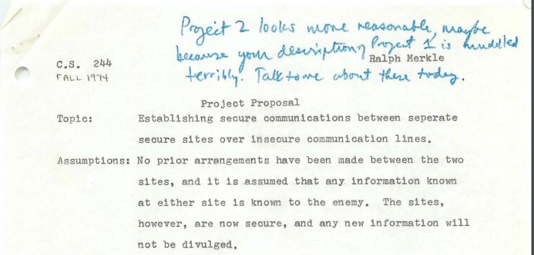
\includegraphics[width=\textwidth, height=0.25\paperheight, keepaspectratio]{../figure/merkle-proposal.png}
\caption{Ralph Merkle's Berkeley CS 224 project proposal for developing
public key cryptography}
\label{merklefig}
\end{figure}

We only found out much later that in the late 1960's, a few years before
Merkle, James Ellis of the British Intelligence agency GCHQ was
\href{http://cryptome.org/jya/ellisdoc.htm}{having similar thoughts}.
His curiosity was spurred by an old World War II manuscript from Bell
labs that suggested the following way that two people could communicate
securely over a phone line. Alice would inject noise to the line, Bob
would relay his messages, and then Alice would subtract the noise to get
the signal. The idea is that an adversary over the line sees only the
sum of Alice's and Bob's signals and doesn't know what came from what.
This got James Ellis thinking whether it would be possible to achieve
something like that digitally. As he later recollected, in 1970 he
realized that in principle this should be possible. He could think of an
hypothetical black box \(B\) that on input a ``handle'' \(\alpha\) and
plaintext \(p\) would give a ``ciphertext'' \(c\). There would be a
secret key \(\beta\) corresponding to \(\alpha\) such that feeding
\(\beta\) and \(c\) to the box would recover \(p\). However, Ellis had
no idea how to actually instantiate this box. He and others kept giving
this question as a puzzle to bright new recruits until one of them,
Clifford Cocks, came up in 1973 with a candidate solution loosely based
on the factoring problem; in 1974 another GCHQ recruit, Malcolm
Williamson, came up with a solution using modular exponentiation.

But among all those thinking of public key cryptography, probably the
people who saw the furthest were two researchers at Stanford, Whit
Diffie and Martin Hellman. They realized that with the advent of
electronic communication, cryptography would find new applications
beyond the military domain of spies and submarines. And they understood
that in this new world of many users and point to point communication,
cryptography would need to scale up. They envisioned an object which we
now call ``trapdoor permutation'' though they called it ``one way
trapdoor function'' or sometimes simply ``public key encryption''. This
is a collection of permutations \(\{ p_k \}\) where \(p_k\) is a
permutation over (say) \(\{0,1\}^{|k|}\), and the map
\((x,k)\mapsto p_k(x)\) is efficiently computable \emph{but} the reverse
map \((k,y) \mapsto p_k^{-1}(y)\) is computationally hard. Yet, there is
also some secret key \(s(k)\) (i.e., the ``trapdoor'') such that using
\(s(k)\) it is possible to efficiently compute \(p^{-1}_k\). Their idea
was that using such a trapdoor permutation, Alice who knows \(s(k)\)
would be able to publish \(k\) on some public file such that everyone
who wants to send her a message \(x\) could do so by computing
\(p_k(x)\). (While today we know, due to the work of Goldwasser and
Micali, that such a deterministic encryption is not a good idea, at the
time Diffie and Hellman had amazing intuitions but didn't really have
proper definitions of security.) But they didn't stop there. They
realized that protecting the \emph{integrity} of communication is no
less important than protecting its \emph{secrecy}. Thus, they imagined
that Alice could ``run encryption in reverse'' in order to certify or
\emph{sign} messages. That is, given some message \(m\), Alice would
send the value \(x=p_k^{-1}(h(m))\) (for a hash function \(h\)) as a way
to certify that she endorses \(m\), and every person who knows \(k\)
could verify this by checking that \(p_k(x)=h(m)\).

At this point, Diffie and Hellman were in a position similar to past
physicists, who predicted that a certain particle should exist but had
no experimental verification. Luckily they
\href{http://cr.yp.to/bib/1988/diffie.pdf}{met Ralph Merkle}. His ideas
about a probabilistic \emph{key exchange protocol}, together with a
suggestion from their Stanford colleague
\href{https://profiles.stanford.edu/john-gill}{John Gill}, inspired them
to come up with what today is known as the \emph{Diffie-Hellman Key
Exchange} (unbeknownst to them, a similar protocol was found two years
earlier at GCHQ by Malcolm Williamson). They published their paper
\href{https://www-ee.stanford.edu/~hellman/publications/24.pdf}{``New
Directions in Cryptography''} in 1976, and it is considered to have
brought about the birth of modern cryptography. However, they still
didn't find their elusive trapdoor function. This was done the next year
by Rivest, Shamir and Adleman who came up with the RSA trapdoor
function, which through the framework of Diffie and Hellman yielded not
just encryption but also signatures (this was essentially the same
function discovered earlier by Clifford Cocks at GCHQ, though as far as
I can tell Cocks, Ellis and Williamson did not realize the application
to digital signatures). From this point on began a flurry of advances in
cryptography which hasn't really died down till this day.

\begin{marginfigure}
\centering
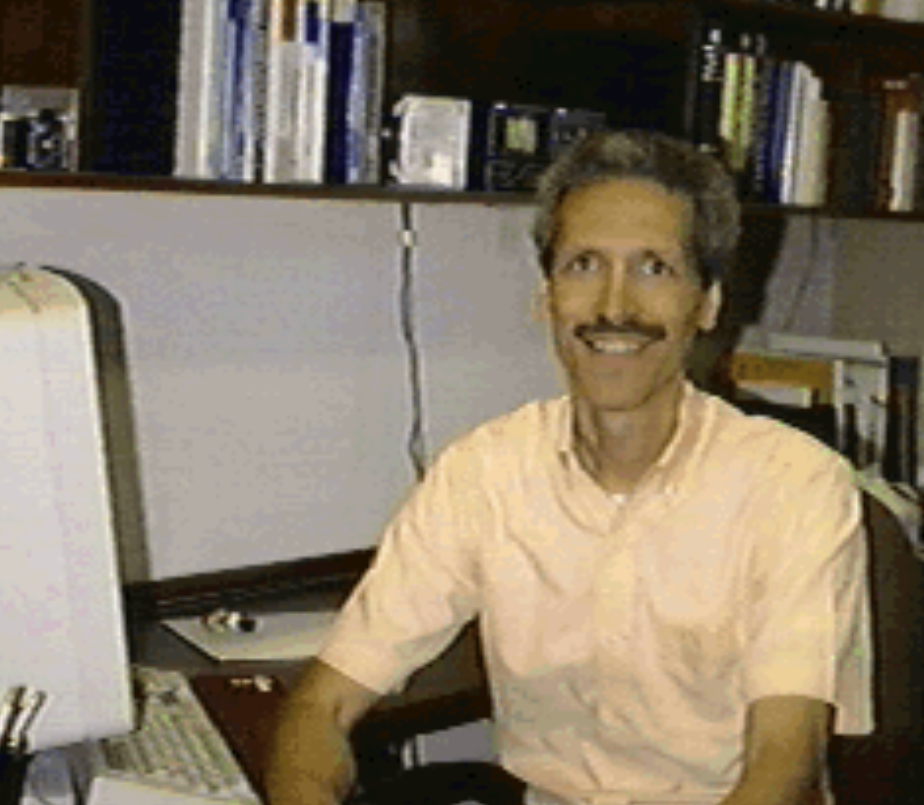
\includegraphics[width=\linewidth, height=1.5in, keepaspectratio]{../figure/john-gill.png}
\caption{John T. Gill III. Gill proposed to Diffie and Hellman to use
modular exponentiation as a one-way function, which (together with
Merkle's ideas) enabled what's known today as the \emph{Diffie-Hellman
Key Exchange} protocol.}
\label{johngillfig}
\end{marginfigure}

\section{Private key crypto recap}\label{10-Private-key-crypto-rec}

Before we embark on the wonderful journey to \emph{public key}
cryptography, let's briefly look back and see what we learned about
\emph{private key cryptography}. This material is mostly covered in
Chapters 1 to 9 of the Katz Lindell (KL) book and Part I (Chapters 1-9)
of the Boneh Shoup (BS) book. Now would be a good time for you to read
the corresponding proofs in one or both of these books. It is often
helpful to see the same proof presented in a slightly different way.
Below is a review of some of the various reductions we saw in class,
with pointers to the corresponding sections in the Katz-Lindell (2nd ed)
and Boneh-Shoup books. These are also covered in
\href{https://web.engr.oregonstate.edu/~rosulekm/crypto/}{Rosulek's
book}.

\begin{itemize}
\tightlist
\item
  Pseudorandom generators (PRG) length extension (from \(n+1\) output
  PRG to \(poly(n)\) output PRG): KL 7.4.2, BS 3.4.2
\item
  PRG's to pseudorandom functions (PRF's): KL 7.5, BS 4.6
\item
  PRF's to Chosen Plaintext Attack (CPA) secure encryption: KL 3.5.2, BS
  5.5
\item
  PRF's to secure Message Authentication Codes (MAC's): KL 4.3, BS 6.3
\item
  MAC's + CPA secure encryption to chosen ciphertext attack (CCA) secure
  encryption: BS 4.5.4, BS 9.4
\item
  Pseudorandom permutation (PRP's) to CPA secure encryption / block
  cipher modes: KL 3.5.2, KL 3.6.2, BS 4.1, 4.4, 5.4
\item
  Hash function applications: fingerprinting, Merkle trees, passwords:
  KL 5.6, BS Chapter 8
\item
  Coin tossing over the phone: we saw a construction in class that used
  a \emph{commitment scheme} built out of a pseudorandom generator. This
  is shown in BS 3.12, KL 5.6.5 shows an alternative construction using
  random oracles.
\item
  PRP's from PRF's: we only sketched the construction which can be found
  in KL 7.6 or BS 4.5
\end{itemize}

One major point we did \emph{not} talk about in this course was
\emph{one way functions}. The definition of a one way function is quite
simple:

\hypertarget{owfdef}{}
\begin{definition}[One Way Functions] \label[definition]{owfdef}

A function \(f:\{0,1\}^*\rightarrow\{0,1\}^*\) is a \emph{one way
function} if it is efficiently computable and for every \(n\) and a
\(poly(n)\) time adversary \(A\), the probability over
\(x\leftarrow_R\{0,1\}^n\) that \(A(f(x))\) outputs \(x'\) such that
\(f(x')=f(x)\) is negligible.

\end{definition}

The ``OWF conjecture'' is the conjecture that one way functions exist.
It turns out to be a necessary and sufficient condition for much of
private key cryptography. That is, the following theorem is known (by
combining works of many people):

\hypertarget{privkeydef}{}
\begin{theorem}[One way functions and private key cryptography] \label[theorem]{privkeydef}

The following are equivalent:

\begin{itemize}
\item
  One way functions exist
\item
  Pseudorandom generators (with non-trivial stretch) exist
\item
  Pseudorandom functions exist
\item
  CPA secure private key encryptions exist
\item
  CCA secure private key encryptions exist
\item
  Message Authentication Codes exist
\item
  Commitment schemes exist
\end{itemize}

\end{theorem}

The key result in the proof of this theorem is the result of Hastad,
Impagliazzo, Levin and Luby that if one way functions exist then
pseudorandom generators exist. If you are interested in finding out
more, see Chapter 7 in
\href{https://people.seas.harvard.edu/~salil/pseudorandomness/}{Vadhan's
pseudorandomness monograph}. Sections 7.2-7.4 in the KL book also cover
a special case of this theorem for the case that the one way function is
a \emph{permutation} on \(\{0,1\}^n\) for every \(n\). This proof has
been considerably simplified and quantitatively improved in works of
Haitner, Holenstein, Reingold, Vadhan, Wee and Zheng. See
\href{http://people.seas.harvard.edu/~salil/research/CompEnt-abs.html}{this
talk of Salil Vadhan} for more on this. See also
\href{http://www.cs.princeton.edu/courses/archive/spring08/cos598D/scribe3.pdf}{these
lecture notes} from a Princeton seminar I gave on this topic (though the
proof has been simplified since then by the above works).

\hypertarget{privkeyattacks}{}
\begin{remark}[Cryptanalytic attacks on private key cryptosystems] \label[remark]{privkeyattacks}

Another topic we did not discuss in depth is attacks on private key
cryptosystems. These attacks often work by ``opening the black box'' and
looking at the internal operation of block ciphers or hash functions. We
then assign variables to various internal registers, and look to find
collections of inputs that would satisfy some non-trivial relation
between those variables. This is a rather vague description, but you can
read KL Section 6.2.6 on \emph{linear} and \emph{differential}
cryptanalysis and BS Sections 3.7-3.9 and 4.3 for more information. See
also \href{http://www.cs.tau.ac.il/~tromer/SKC2006/}{this course of Adi
Shamir}, and the courses of Dunkelman on analyzing
\href{https://www.cs.haifa.ac.il/~orrd/BlockCipherSeminar/}{block
ciphers} and
\href{https://www.cs.haifa.ac.il/~orrd/HashFuncSeminar/}{hash
functions}. There is also the fascinating area of \emph{side channel}
attacks on both public and private key crypto, see
\href{http://www.cs.tau.ac.il/~tromer/istvr1516.html}{this course of
Tromer}.

\end{remark}

\hypertarget{signaturesrem}{}
\begin{remark}[Digital Signatures] \label[remark]{signaturesrem}

We will discuss in this lecture \emph{Digital signatures}, which are the
public key analog of message authentication codes. Surprisingly, despite
being a ``public key'' object, it is possible to base digital signatures
on one-way functions (this is obtained using ideas of Lamport, Merkle,
Goldwasser-Goldreich-Micali, Naor-Yung, and Rompel). However these
constructions are not very efficient (and this may be inherent), and so
in practice people use digital signatures that are built using similar
techniques to those used for public key encryption.

\end{remark}

\section{Public Key Encryptions:
Definition}\label{10-Public-Key-Encryptions}

We now discuss how we define security for public key encryption. As
mentioned above, it took quite a while for cryptographers to arrive at
the ``right'' definition, but in the interest of time we will skip ahead
to what by now is the standard basic notion (see also \cref{PKCfig}):

\begin{marginfigure}
\centering
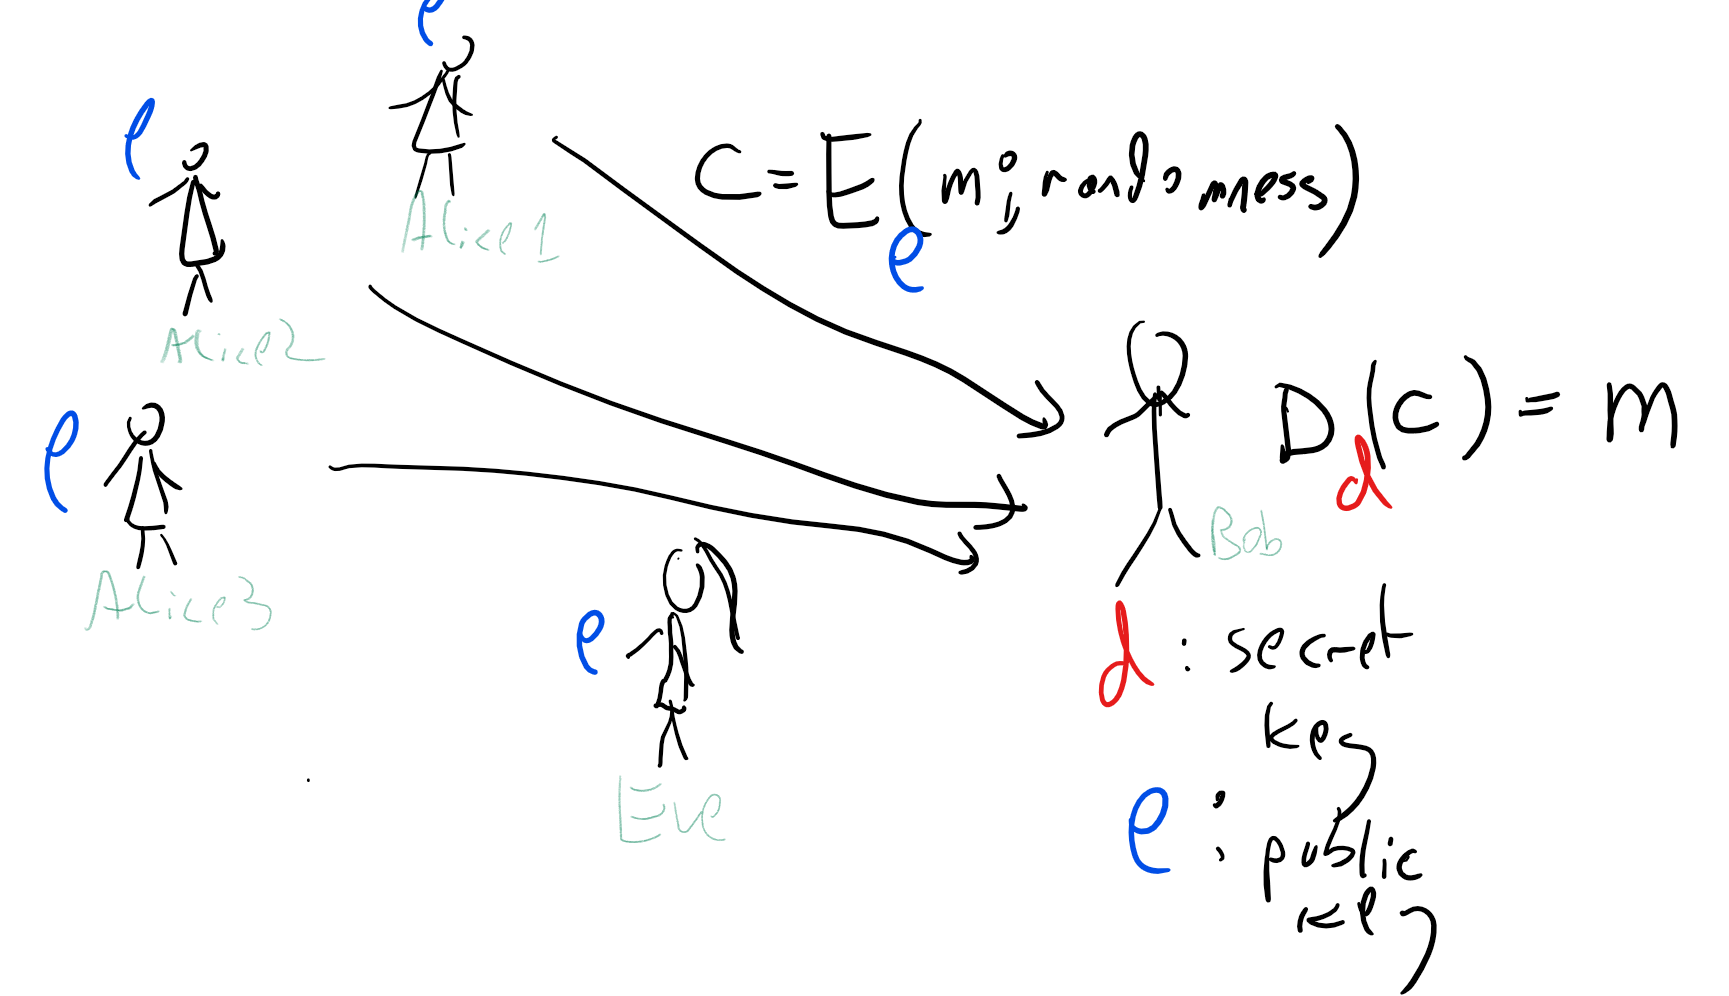
\includegraphics[width=\linewidth, height=1.5in, keepaspectratio]{../figure/pkenccartoon.png}
\caption{In a public key encryption, the receiver Bob generates a
\emph{pair} of keys \((e,d)\). The \emph{encryption key} \(e\) is used
for encryption, and the \emph{decryption key} is used for decryption. We
call it a public key system since the security of the scheme does not
rely on the adversary Eve not knowing the encryption key. Hence, Bob can
publicize the key \(e\) to a great many potential receivers and still
ensure confidentiality of the messages he receives.}
\label{PKCfig}
\end{marginfigure}

\hypertarget{pubkeydef}{}
\begin{definition}[Valid public key encryption] \label[definition]{pubkeydef}

A triple of efficient algorithms \((G,E,D)\) is a \emph{public key
encryption scheme} of length function \(\ell:\N \rightarrow \N\) if it
satisfies the following:

\begin{itemize}
\item
  \(G\) is a probabilistic algorithm known as the \emph{key generation
  algorithm} that on input \(1^n\) outputs a distribution over pair of
  keys \((e,d)\).\\
\item
  \(E\) is the \emph{encryption algorithm} that takes a pair of inputs
  \(e,m\) with \(m\in \{0,1\}^{\ell(n)}\) and outputs \(c=E_e(m)\).\\
\item
  \(D\) is the \emph{decryption algorithm} that takes a pair of inputs
  \(d,c\) and outputs \(m'=D_d(c)\).\\
\item
  For every \(m\in\{0,1\}^{\ell(n)}\), with probability \(1-negl(n)\)
  over the choice of \((e,d)\) output from \(G(1^n)\) and the coins of
  \(E\),\(D\), \(D_d(E_e(m))=m\).\\
\end{itemize}

\end{definition}

\cref{pubkeydef} just refers to the \emph{validity} of a public-key
encryption scheme, namely the condition that we can encrypt and decrypt
using the keys \(e\) and \(d\) respectively, but not to its security.
The standard definition of security for public-key encryption is CPA
security:

\hypertarget{cpasecpubkeydef}{}
\begin{definition}[CPA security for public-key encryption] \label[definition]{cpasecpubkeydef}

We say that \((G,E,D)\) is \emph{CPA secure} if every efficient
adversary \(A\) wins the following game with probability at most
\(1/2+negl(n)\):

\begin{itemize}
\item
  \((e,d) \leftarrow_R G(1^n)\)
\item
  \(A\) is given \(e\) and outputs a pair of messages
  \(m_0,m_1 \in \{0,1\}^n\).
\item
  \(A\) is given \(c=E_e(m_b)\) for \(b\leftarrow_R\{0,1\}\).
\item
  \(A\) outputs \(b'\in\{0,1\}\) and \emph{wins} if \(b'=b\).
\end{itemize}

\end{definition}

\begin{pause} \label[pause]{10-Despite-it-being-a-cho}

Despite it being a ``chosen plaintext attack'', we don't explicitly give
\(A\) access to the encryption oracle in the public key setting. Make
sure you understand why giving it such access would not give it more
power.

\end{pause}

One metaphor for a public key encryption is a ``self-locking lock''
where you don't need the key to \emph{lock it} (but rather you simply
push the shackle until it clicks and lock), but you do need the key to
\emph{unlock} it. So, if Alice generates \((e,d)=G(1^n)\), then \(e\)
serves as the ``lock'' that can be used to \emph{encrypt} messages for
Alice while only \(d\) can be used to \emph{decrypt} the messages.
Another way to think about it is that \(e\) is a ``hobbled key'' that
can be used for only some of the functions of \(d\).

\subsection{The obfuscation paradigm}\label{10-The-obfuscation-paradi}

Why would someone imagine that such a magical object could exist? The
writing of both James Ellis as well as Diffie and Hellman suggests that
their thought process was roughly as follows. You imagine a ``magic
black box'' \(B\) such that if all parties have access to \(B\) then we
could get a public key encryption scheme. Now if public key encryption
was impossible it would mean that for every possible program \(P\) that
computes the functionality of \(B\), if we distribute the code of \(P\)
to all parties, then we don't get a secure encryption scheme. That means
that \emph{no matter what program \(P\) the adversary gets}, she will
always be able to get some information out of that code that helps break
the encryption, even though she wouldn't have been able to break it if
\(P\) was a black box. Now, intuitively understanding arbitrary code is
a very hard problem, so Diffie and Hellman imagined that it might be
possible to take this ideal \(B\) and compile it to some sufficiently
low level assembly language so that it would behave as a ``virtual black
box''.

In particular, if you took, say, the encoding procedure
\(m \mapsto p_k(m)\) of a block cipher with a particular key \(k\) and
ran it through an optimizing compiler, you might hope that while it
would be possible to perform this map using the resulting executable, it
will be hard to extract \(k\) from it. Hence, you could treat this code
as a ``public key''. This suggests the following approach for getting an
encryption scheme:

\begin{quote} \label[quote]{10-Obfuscation-based-publ}

\textbf{``Obfuscation based public key encryption'':} (Thought
experiment - not an actual construction)

\textbf{Ingredients:}

\emph{(i)} A pseudorandom permutation collection
\(\{ p_k \}_{k\in \{0,1\}^*}\) where for every \(k\in \{0,1\}^n\),
\(p_k:\{0,1\}^n \rightarrow \{0,1\}^n\)

\emph{(ii)} An ``obfuscating compiler'' polynomial-time computable
\(O:\{0,1\}^* \rightarrow \{0,1\}^*\) such that for every circuit \(C\),
\(O(C)\) is a circuit that computes the same function as \(C\).

\textbf{Operation:}

\begin{itemize}
\item
  \emph{Key Generation:} The private key is
  \(k \leftarrow_R \{0,1\}^n\), the public key is \(E=O(C_k)\) where
  \(C_k\) is the circuit that maps \(x\in \{0,1\}^n\) to \(p_k(x)\).
\item
  \emph{Encryption:} To encrypt \(m\in \{0,1\}^n\) with public key
  \(E\), choose \(\ensuremath{\mathit{IV}} \leftarrow_R \{0,1\}^n\) and
  output
  \((\ensuremath{\mathit{IV}}, E(x \oplus \ensuremath{\mathit{IV}}))\).
\item
  \emph{Decryption:} To decrypt \((\ensuremath{\mathit{IV}},y)\) with
  key \(k\), output \(\ensuremath{\mathit{IV}} \oplus p_k^{-1}(y)\).
\end{itemize}

\end{quote}

Diffie and Hellman couldn't really find a way to make this work, but it
convinced them this notion of public key is not \emph{inherently
impossible}. This concept of compiling a program into a functionally
equivalent but ``inscrutable'' form is known as \emph{software
obfuscation}. It had turned out to be quite a tricky object to both
define formally and achieve, but it serves as very good intuition for
what can be achieved, even if, as with the random oracle, this intuition
can sometimes be too optimistic. (Indeed, if software obfuscation was
possible then we could obtain a ``random oracle like'' hash function by
taking the code of a function \(f_k\) chosen from a PRF family and
compiling it through an obfuscating compiler.)

We will not formally define obfuscators yet, but on an intuitive level
it would be a compiler that takes a program \(P\) and maps into a
program \(P'\) such that:

\begin{itemize}
\tightlist
\item
  \(P'\) is not much slower/bigger than \(P\) (e.g., as a Boolean
  circuit it would be at most polynomially larger).
\item
  \(P'\) is functionally equivalent to \(P\), i.e., \(P'(x)=P(x)\) for
  every input \(x\).\footnote{For simplicity, assume that the program
    \(P\) is \emph{side effect free} and hence it simply computes some
    function, say from \(\{0,1\}^n\) to \(\{0,1\}^\ell\) for some
    \(n,\ell\).}
\item
  \(P'\) is ``inscrutable'' in the sense that seeing the code of \(P'\)
  is not more informative than getting \emph{black box access} to \(P\).
\end{itemize}

Let me stress again that there is no known construction of obfuscators
achieving something similar to this definition. In fact, the most
natural formalization of this definition is
\href{https://www.boazbarak.org/Papers/obfuscate.pdf}{impossible} to
achieve (as we might see later in this course). Only very recently
(exciting!) progress was finally made towards obfuscators-like notions
strong enough to achieve these and other applications, and there are
some significant caveats, see \href{https://eprint.iacr.org/2016/210}{my
survey on this topic} and a more recent
\href{https://www.quantamagazine.org/computer-scientists-achieve-crown-jewel-of-cryptography-20201110/}{Quanta
article}.

However, when trying to stretch your imagination to consider the amazing
possibilities that could be achieved in cryptography, it is not a bad
heuristic to first ask yourself what could be possible if only everyone
involved had access to a magic black box. It certainly worked well for
Diffie and Hellman.

\section{Some concrete candidates:}\label{10-Some-concrete-candidat}

We would have loved to prove a theorem of the form:

\begin{quote}
\textbf{``Theorem'':} If the PRG conjecture is true, then there exists a
CPA-secure public key encryption.
\end{quote}

This would have meant that we do not need to assume anything more than
the already minimal notion of pseudorandom generators (or equivalently,
one way functions) to obtain public key cryptography. Unfortunately, no
such result is known (and this may be
\href{https://www.cs.virginia.edu/~mohammad/files/papers/MerkleFull.pdf}{inherent}).
The kind of results we know have the following form:

\begin{quote}
\textbf{Theorem:} If problem \(X\) is hard, then there exists a
CPA-secure public key encryption.
\end{quote}

Here, \(X\) is some problem that people have tried to solve and
couldn't. Thus, we have various \emph{candidates} for public key
encryption, and we fervently hope that at least one of them is actually
secure. The \href{https://eprint.iacr.org/2017/365.pdf}{dirty little
secret} of cryptography is that we actually don't have that many
candidates. We really have only two well studied families.\footnote{There
  have been some other more exotic suggestions for public key encryption
  (including some by
  \href{http://www.eng.tau.ac.il/~bennyap/pubs/ncpkcFull1.pdf}{yours
  truly} as well as suggestions such as the
  \href{http://eprint.iacr.org/2006/291}{isogeny star problem}, though
  see also \href{http://arxiv.org/pdf/1012.4019.pdf}{this}), but they
  have not yet received wide scrutiny.} One is the ``group theoretic''
family that relies on the difficulty of the discrete logarithm (over
modular arithmetic or elliptic curves) or the integer factoring problem.
The other is the ``coding/lattice theoretic'' family that relies on the
difficulty of solving noisy linear equations or related problems such as
finding short vectors in a \emph{lattice} and solving instances of the
``knapsack'' problem. Moreover, problems from the first family are known
to be \emph{efficiently solvable} in a computational model known as
``quantum computing''. If large scale physical devices that simulate
this model, known as \emph{quantum computers}, exist, then they could
break all cryptosystems relying on these problems, and we'll be down to
only having a \emph{single} family of candidate public key encryption
schemes.

We will start by describing cryptosystems based on the first family
(which was discovered before the other and was more widely implemented),
and talk about the second family in future lectures.

\subsection{Diffie-Hellman Encryption (aka
El-Gamal)}\label{10-Diffie-Hellman-Encrypt}

The Diffie-Hellman public key system is built on the presumed difficulty
of the \emph{discrete logarithm problem}:

For any number \(p\), let \(\Z_p\) be the set of numbers
\(\{0,\ldots,p-1\}\) where addition and multiplication are done modulo
\(p\). We will think of numbers \(p\) that are of magnitude roughly
\(2^n\), so they can be described with about \(n\) bits. We can clearly
multiply and add such numbers modulo \(p\) in \(poly(n)\) time. If
\(g\in \Z_p\) and \(a\) is any natural number, we can define \(g^a\) to
be simply \(g\cdot g \cdots g\) (\(a\) times). A priori one might think
that it would take \(a\cdot poly(n)\) time to compute \(g^a\), which
might be exponential if \(a\) itself is roughly \(2^n\). However, we can
compute this in \(poly((\log a) \cdot n)\) time using the \emph{repeated
squaring trick}. The idea is that if \(a=2^{\ell}\), then we can compute
\(g^a\) in \(\ell\) by squaring \(g\) \(\ell\) times, and a general
\(a\) can be decomposed into powers of two using the binary
representation.

The \emph{discrete logarithm} problem is the problem of computing, given
\(g,h \in \Z_p\), a number \(a\) such that \(g^a=h\). If such a solution
\(a\) exists then there is always also a solution of size at most \(p\)
(can you see why?) and so the solution can be represented using \(n\)
bits. However, currently the best-known algorithm for computing the
discrete logarithm runs in time roughly \(2^{n^{1/3}}\), which is
currently prohibitively expensive when \(p\) is a prime of length about
\(2048\) bits.\footnote{The running time of the best known algorithms
  for computing the discrete logarithm modulo \(n\) bit primes is
  \(2^{f(n)2^{n^{1/3}}}\), where \(f(n)\) is a function that depends
  polylogarithmically on \(n\). If \(f(n)\) would equal \(1\), then we'd
  need numbers of \(128^3 \approx 2\cdot 10^6\) bits to get \(128\) bits
  of security, but because \(f(n)\) is larger than one, the current
  \href{https://goo.gl/ntszsg}{estimates} are that we need to let
  \(n=3072\) bit key to get \(128\) bits of of security. Still, the
  existence of such a non-trivial algorithm means that we need much
  larger keys than those used for private key systems to get the same
  level of security. In particular, to double the estimated security to
  \(256\) bits, NIST recommends that we multiply the RSA keysize
  five-fold to \(15,360\). (The same document also says that SHA-256
  gives \(256\) bits of security as a pseudorandom generator but only
  \(128\) bits when used to hash documents for digital signatures; can
  you see why?)}

John Gill suggested to Diffie and Hellman that modular exponentiation
can be a good source for the kind of ``easy-to-compute but
hard-to-invert'' functions they were looking for. Diffie and Hellman
based a public key encryption scheme as follows:

\begin{itemize}
\tightlist
\item
  The \emph{key generation algorithm}, on input \(n\), samples a prime
  number \(p\) of \(n\) bits description (i.e., between \(2^{n-1}\) to
  \(2^n\)), a number \(g\leftarrow_R \Z_p\) and
  \(a \leftarrow_R \{0,\ldots,p-1\}\). We also sample a hash function
  \(H:\{0,1\}^n\rightarrow\{0,1\}^\ell\). The public key \(e\) is
  \((p,g,g^a,H)\), while the secret key \(d\) is \(a\).\footnote{Formally,
    the secret key should contain all the information in the public key
    plus the extra secret information, but we omit the public
    information for simplicity of notation.}
\end{itemize}

\begin{itemize}
\item
  The \emph{encryption algorithm}, on input a message
  \(m \in \{0,1\}^\ell\) and a public key \(e=(p,g,h,H)\), will choose a
  random \(b\leftarrow_R \{0,\ldots,p-1\}\) and output
  \((g^b,H(h^b)\oplus m)\).
\item
  The \emph{decryption algorithm}, on input a ciphertext \((f,y)\) and
  the secret key, will output \(H(f^a) \oplus y\).
\end{itemize}

The correctness of the decryption algorithm follows from the fact that
\((g^a)^b = (g^b)^a = g^{ab}\) and hence \(H(h^b)\) computed by the
encryption algorithm is the same as the value \(H(f^a)\) computed by the
decryption algorithm. A simple relation between the discrete logarithm
and the Diffie-Hellman system is the following:

\hypertarget{dhinseclem}{}
\begin{lemma} \label[lemma]{dhinseclem}

If there is a polynomial time algorithm for the discrete logarithm
problem, then the Diffie-Hellman system is \emph{insecure}.

\end{lemma}

\begin{proof} \label[proof]{10-Using-a-discrete-logar}

Using a discrete logarithm algorithm, we can compute the private key
\(a\) from the parameters \(p,g,g^a\) present in the public key, and
clearly once we know the private key we can decrypt any message of our
choice.

\end{proof}

Unfortunately, no such result is known in the other direction. However
in the random oracle model, we can prove that this protocol is secure in
the random-oracle model, under the assumption that the task of computing
\(g^{ab}\) from \(g^a\) and \(g^b\) (which is now known as the
\emph{Diffie-Hellman problem}) is hard.

\begin{quote}
\textbf{Computational Diffie-Hellman Assumption:} Let \(\mathbb{G}\) be
a group whose elements can be described in \(n\) bits, with an
associative and commutative multiplication operation that can be
computed in \(poly(n)\) time. The \emph{Computational Diffie-Hellman
(CDH)} assumption holds with respect to the group \(\mathbb{G}\) if for
every generator (see below) \(g\) of \(\mathbb{G}\) and efficient
algorithm \(A\), the probability that on input \(g,g^a,g^b\), \(A\)
outputs the element \(g^{ab}\) is negligible as a function of
\(n\).\footnote{Formally, since it is an asymptotic statement, the CDH
  assumption needs to be defined with a \emph{sequence of groups}.
  However, to make notation simpler we will ignore this issue, and use
  it only for groups (such as the numbers modulo some \(n\) bit primes)
  where we can easily increase the ``security parameter'' \(n\).}
\end{quote}

In particular we can make the following conjecture:

\begin{quote}
\textbf{Computational Diffie-Hellman Conjecture for mod prime groups:}
For a random \(n\)-bit prime and random \(g \in \mathbb{Z}_p\), the CDH
holds with respect to the group
\(\mathbb{G} = \{ g^a \mod p \;| a\in \mathbb{Z} \}\).
\end{quote}

That is, for every polynomial \(q:\N \rightarrow \N\), if \(n\) is large
enough, then with probability at least \(1-1/q(n)\) over the choice of a
uniform prime \(p\in [2^n]\) and \(g\in \Z_p\), for every circuit \(A\)
of size at most \(q(n)\), the probability that \(A(g,p,g^a,g^b)\)
outputs \(h\) such that \(g^{ab} = h \mod p\) is at most \(1/q(n)\)
where the probability is taken over \(a,b\) chosen at random in
\(\Z_p\). (In practice people often take \(g\) to be a generator of a
group significantly smaller in size than \(p\), which enables \(a,b\) to
be smaller numbers and hence multiplication to be more efficient; We
ignore this optimization in our discussions.)

\begin{pause} \label[pause]{10-Please-take-your-time-}

Please take your time to re-read the following conjecture until you are
sure you understand what it means. Victor Shoup's excellent and online
available book \href{http://www.shoup.net/ntb/}{A Computational
Introduction to Number Theory and Algebra} has an in depth treatment of
groups, generators, and the discrete log and Diffie-Hellman problem. See
also Chapters 10.4 and 10.5 in the Boneh-Shoup book, and Chapters 8.3
and 11.4 in the Katz-Lindell book. There are also solved group theory
exercises at the end of this chapter.

\end{pause}

\hypertarget{DHROMthm}{}
\begin{theorem}[Diffie-Hellman security in Random Oracle Model] \label[theorem]{DHROMthm}

Suppose that the Computational Diffie-Hellman Conjecture for mod prime
groups is true. Then, the Diffie-Hellman public key encryption is CPA
secure in the random oracle model.

\end{theorem}

\begin{proof} \label[proof]{10-For-CPA-security-we-ne}

For CPA security we need to prove that (for fixed \(\mathbb{G}\) of size
\(p\) and random oracle \(H\)) the following two distributions are
computationally indistinguishable for every two strings
\(m,m' \in \{0,1\}^\ell\):

\begin{itemize}
\item
  \((g^a,g^b,H(g^{ab})\oplus m)\) for \(a,b\) chosen uniformly and
  independently in \(\Z_{p}\).
\item
  \((g^a,g^b,H(g^{ab})\oplus m')\) for \(a,b\) chosen uniformly and
  independently in \(\Z_{p}\).
\end{itemize}

(can you see why this implies CPA security? you should pause here and
verify this!)

We make the following claim:

\textbf{CLAIM:} For a fixed \(\mathbb{G}\) of size \(p\), generator
\(g\) for \(\mathbb{G}\), and given random oracle \(H\), if there is a
size \(T\) distinguisher \(A\) with \(\epsilon\) advantage between the
distribution \((g^a,g^b,H(g^{ab}))\) and the distribution
\((g^a,g^b,U_\ell)\) (where \(a,b\) are chosen uniformly and
independently in \(\Z_{p}\)), then there is a size \(poly(T)\) algorithm
\(A'\) to solve the Diffie-Hellman problem with respect to
\(\mathbb{G},g\) with success at least \(\epsilon\). That is, for random
\(a,b \in \Z_p\), \(A'(g,g^a,g^b)=g^{ab}\) with probability at least
\(\epsilon/(2T)\).

\textbf{Proof of claim:} The proof is simple. We claim that under the
assumptions above, \(a\) makes the query \(g^{ab}\) to its oracle \(H\)
with probability at least \(\epsilon/2\) since otherwise, by the ``lazy
evaluation'' paradigm, we can assume that \(H(g^{ab})\) is chosen
independently at random after \(A\)'s attack is completed and hence
(conditioned on the adversary not making that query), the value
\(H(g^{ab})\) is indistinguishable from a uniform output. Therefore, on
input \(g,g^a,g^b\), \(A'\) can simulate \(A\) and simply output one of
the at most \(T\) queries that \(A\) makes to \(H\) at random and will
be successful with probability at least \(\epsilon/(2T)\).

Now given the claim, we can complete the proof of security via the
following hybrids. Define the following ``hybrid'' distributions (where
in all cases \(a,b\) are chosen uniformly and independently in
\(\Z_{p}\)):

\begin{itemize}
\item
  \(H_0\): \((g^a,g^b,H(g^{ab}) \oplus m)\)
\item
  \(H_1\): \((g^a,g^b,U_\ell \oplus m)\)
\item
  \(H_2\): \((g^a,g^b,U_\ell \oplus m')\)
\item
  \(H_3\): \((g^a,g^b,H(g^{ab}) \oplus m')\)
\end{itemize}

The claim implies that \(H_0 \approx H_1\). Indeed otherwise we could
transform a distinguisher \(T\) between \(H_0\) and \(H_1\) to a
distinguisher \(T'\), violating the claim by letting
\(T'(h,h',z) = T(h,h',z \oplus m)\).

The distributions \(H_1\) and \(H_2\) are \emph{identical} by the same
argument as the security of the one time pad (since \(U_\ell \oplus m\)
is identical to \(U_\ell\)).

The distributions \(H_2\) and \(H_3\) are computationally
indistinguishable by the same argument that \(H_0 \approx H_1\).

Together these imply that \(H_0 \approx H_3\) which yields the CPA
security of the scheme.

\end{proof}

\hypertarget{ddhrem}{}
\begin{remark}[Decisional Diffie Hellman] \label[remark]{ddhrem}

One can get security results for this protocol without a random oracle
if we assume a stronger variant known as the \emph{Decisional
Diffie-Hellman (DDH)} assumption: for a random
\(a,b, u \in \mathbb{Z}_p\) (prime \(p\)), the triple
\((g^a, g^b, g^{ab})\approx (g^a, g^b, g^u)\). This implies CDH (can you
see why?). DDH also restricts our focus to groups of prime order. In
particular, DDH does not hold in even-order groups. For example, DDH
does not hold in \(\mathbb{Z}^{\*}_p=\{1,2\ldots p-1\}\) (with group
operation multiplication mod \(p\)) since half of its elements are
quadratic residues \emph{and} it is efficient to test if an element is a
quadratic residue using Fermat's little theorem (can you see why? See
Exercise 10.7). However, DDH holds in subgroups of \(\mathbb{Z}^{\*}_p\)
of prime order. If \(p\) is a safe prime (i.e.~\(p=2q+1\) for a prime
\(q\)), then we can instead use the subgroup of quadratic residues,
which has prime order \(q\). See Boneh-Shoup 10.4.1 for more details on
the underlying groups for CDH and DDH.

\end{remark}

\hypertarget{curverem}{}
\begin{remark}[Elliptic curve cryptography] \label[remark]{curverem}

As mentioned, the Diffie-Hellman systems can be run with many variants
of Abelian groups. Of course, for some of those groups the discrete
logarithm problem might be easy, and so they would be inappropriate to
use for this system. One variant that has been proposed is
\href{https://en.wikipedia.org/wiki/Elliptic_curve_cryptography}{elliptic
curve cryptography}. This is a group consisting of points of the form
\((x,y,z)\in \Z_p^3\) that satisfy a certain equation, and
multiplication can be defined according in a certain way. The main
advantage of elliptic curve cryptography is that the best known
algorithms run in time \(2^{\approx n}\) as opposed to
\(2^{\approx n^{1/3}}\), which allows for much shorter keys.
Unfortunately, elliptic curve cryptography is just as susceptible to
quantum algorithms as the discrete logarithm problem over \(\Z_p\).

\end{remark}

\hypertarget{DHKErem}{}
\begin{remark}[Encryption vs Key Exchange and El Gamal] \label[remark]{DHKErem}

In most of the cryptography literature the protocol above is called the
\emph{Diffie-Hellman Key Exchange} protocol, and when considered as a
public key system it is sometimes known as \emph{ElGamal
encryption}.\footnote{ElGamal's actual contribution was to design a
  \emph{signature scheme} based on the Diffie-Hellman problem, a variant
  of which is the Digital Signature Algorithm (DSA) described below.}
The reason for this mostly stems from the early confusion on what the
right security definitions are. Diffie and Hellman thought of encryption
as a \emph{deterministic} process and so they called their scheme a
``key exchange protocol''. The work of Goldwasser and Micali showed that
encryption must be probabilistic for security. Also, because of
efficiency considerations, these days public key encryption is mostly
used as a mechanism to exchange a key for a private key encryption that
is then used for the bulk of the communication. Together this means that
there is not much point in distinguishing between a two-message key
exchange algorithm and a public key encryption.

\end{remark}

\subsection{Sampling random primes}\label{10-Sampling-random-primes}

To sample a random \(n\) bit prime, one can sample a random number
\(0 \leq p < 2^n\) and then test if \(p\) is prime. If it is not prime,
then we can sample a new random number again. To make this work we need
to show two properties:

\emph{Efficient testing:} That there is a \(poly(n)\) time algorithm to
test whether an \(n\) bit number is a prime. It turns out that there are
such \href{https://en.wikipedia.org/wiki/Primality_test}{known
algorithms}. \emph{Randomized} algorithm have been known since the
1970's. Moreover in a 2002 breakthrough,
\href{https://goo.gl/nycWFA}{Manindra Agrawal, Neeraj Kayal, and Nitin
Saxena} (a professor and two undergraduate students from the Indian
Institute of Technology Kanpur) came up with the first deterministic
polynomial time algorithm for testing primality.

\emph{Prime density:} That the probability that a random \(n\) bit
number is prime is at least \(1/poly(n)\). This probability is in fact
\(1/\ln(2^n)=\Omega(1/n)\) by the \href{https://goo.gl/ChrXJY}{Prime
Number Theorem}. However, for the sake of completeness, we sketch below
a simple argument showing the probability is at least \(\Omega(1/n^2)\).

\hypertarget{primedensitylem}{}
\begin{lemma} \label[lemma]{primedensitylem}

The number of primes between \(1\) and \(N\) is \(\Omega(N/\log N)\).

\end{lemma}

\begin{proof} \label[proof]{10-Recall-that-the-least-}

Recall that the \emph{least common multiple (LCM)} of two or more
\(a_1,\ldots,a_t\) is the smallest number that is a multiple of all of
the \(a_i\)'s. One way to compute the LCM of \(a_1,\ldots,a_t\) is to
take the prime factorizations of all the \(a_i\)'s, and then the LCM is
the product of all the primes that appear in these factorizations, each
taken to the corresponding highest power that appears in the
factorization. Let \(k\) be the number of primes between \(1\) and
\(N\). The lemma will follow from the following two claims:

\textbf{CLAIM 1:} \(\ensuremath{\mathit{LCM}}(1,\ldots,N) \leq N^k\).

\textbf{CLAIM 2:} If \(N\) is odd, then
\(\ensuremath{\mathit{LCM}}(1,\ldots,N) \geq 2^{N-1}\).

The two claims immediately imply the result, since they imply that
\(2^N \leq N^k\), and taking logs we get that \(N-2 \leq k \log N\) or
\(k \geq (N-2)/\log N\). (We can assume that \(N\) is odd without of
loss of generality, since changing from \(N\) to \(N+1\) can change the
number of primes by at most one.) Thus, all that is left is to prove the
two claims.

\textbf{Proof of CLAIM 1:} Let \(p_1,\ldots,p_k\) be all the prime
numbers between \(1\) and \(N\), and let \(e_i\) be the largest integer
such that \(p_i^{e_i} \leq N\) and \(L = p_1^{e_1} \cdots p_k^{e_k}\).
Since \(L\) is the product of \(k\) terms, each of size at most \(N\),
\(L \leq N^k\). But we claim that every number \(1 \leq a \leq N\)
divides \(L\). Indeed, every prime \(p\) in the prime factorization of
\(a\) is one of the \(p_i\)'s, and since \(a \leq N\), the power in
which \(p\) appears in \(a\) is at most \(e_i\). By the definition of
the least common multiple, this means that
\(\ensuremath{\mathit{LCM}}(1,\ldots,N) \leq L\). QED (CLAIM 1)

\textbf{Proof of CLAIM 2:} Consider the integral
\(I=\int_0^1 x^{(N-1)/2}(1-x)^{(N-1)/2} dx\). This is clearly some
positive number and so \(I>0\). On one hand, for every \(x\) between
zero and one, \(x(1-x) \leq 1/4\) and hence \(I\) is at most
\(4^{-(N-1)/2}=2^{-N+1}\). On the other hand, the polynomial
\(x^{(N-1)/2}(1-x)^{(N-1)/2}\) is some polynomial of degree at most
\(N-1\) with integer coefficients, and so
\(I=\sum_{k=0}^{N-1} C_k \int_0^1 x^k dx\) for some integer coefficients
\(C_0,\ldots,C_{N-1}\). Since \(\int_0^1 x^k = \tfrac{1}{k+1}\), we see
that \(I\) is a sum of fractions with integer numerators and with
denominators that are at most \(N\). Since all the denominators are at
most \(N\) and \(I>0\), it follows that
\(I \geq \tfrac{1}{LCM(1,\ldots,N)}\), and so
\begin{equation*}
2^{-N+1} \geq I \geq \tfrac{1}{LCM(1,\ldots,N)}
\end{equation*}
which implies \(\ensuremath{\mathit{LCM}}(1,\ldots,N) \leq 2^{N-1}\).
QED (CLAIM 2 and hence lemma)

\end{proof}

\subsection{A little bit of group
theory.}\label{10-A-little-bit-of-group-}

If you haven't seen group theory, it might be useful for you to do a
quick review. We will not use much group theory and mostly use the
theory of finite commutative (also known as Abelian) groups (in fact
often \emph{cyclic}) which are such a baby version that it might not be
considered true ``group theory'' by many group theorists. Shoup's
\href{http://www.shoup.net/ntb/}{excellent book} contains everything we
need to know (and much more than that). What you need to remember is the
following:

\begin{itemize}
\item
  A \emph{finite commutative group} \(\mathbb{G}\) is a finite set
  together with a multiplication operation that satisfies
  \(a\cdot b = b\cdot a\) and
  \((a\cdot b)\cdot c = (a\cdot b)\cdot c)\).
\item
  \(\mathbb{G}\) has a special element known as \(1\), where \(g1=1g=g\)
  for every \(g\in\mathbb{G}\) and for every \(g\in \mathbb{G}\) there
  exists an element \(g^{-1}\in \mathbb{G}\) such that \(gg^{-1}=1\).
\item
  For every \(g\in \mathbb{G}\), the \emph{order} of \(g\), denoted
  \(order(g)\), is the smallest positive integer \(a\) such that
  \(g^a=1\).
\end{itemize}

The following basic facts are all not too hard to prove and would be
useful exercises:

\begin{itemize}
\item
  For every \(g\in \mathbb{G}\), the map \(a \mapsto g^a\) is a \(k\) to
  \(1\) map from \(\{0,\ldots,|\mathbb{G}|-1\}\) to \(\mathbb{G}\) where
  \(k=|\mathbb{G}|/order(g)\). See footnote for hint\footnote{For every
    \(f\in \mathbb{G}\), you can show a one to one and onto mapping
    between the set \(\{ a : g^a = 1 \}\) and the set
    \(\{b : g^b= f \}\) by choosing some element \(b\) from the latter
    set and looking at the map \(a \mapsto a+b \mod |\mathbb{G}|\).}
\item
  As a corollary, the order of \(g\) is always a divisor of
  \(|\mathbb{G}|\). This is a special case of a more general phenomenon:
  the set \(\{ g^a \;|\; a\in\mathbb{Z} \}\) is a subset of the group
  \(\mathbb{G}\) that is closed under multiplication, and such subsets
  are known as \emph{subgroups} of \(\mathbb{G}\). It is not hard to
  show (using the same approach as above) that for every group
  \(\mathbb{G}\) and subgroup \(\mathbb{H}\), the size of \(\mathbb{H}\)
  divides the size of \(\mathbb{G}\). This is known as
  \href{https://goo.gl/Q9VSqn}{Lagrange's Theorem} in group theory.
\item
  An element \(g\) of \(\mathbb{G}\) is called a \emph{generator} if
  \(order(g)=|\mathbb{G}|\). A group is called \emph{cyclic} if it has a
  generator. If \(\mathbb{G}\) is cyclic then there is a (not
  necessarily efficiently computable) \emph{isomorphism}
  \(\phi:\mathbb{G}\rightarrow\Z_{|\mathbb{G}|}\) which is a one-to-one
  and onto map satisfying \(\phi(g\cdot h)=\phi(g)+\phi(h)\) for every
  \(g,h\in\mathbb{G}\).
\end{itemize}

When using a group \(\mathbb{G}\) for the Diffie-Hellman protocol, we
want the property that \(g\) is a \emph{generator} of the group, which
also means that the map \(a \mapsto g^a\) is a one-to-one mapping from
\(\{0,\ldots,|\mathbb{G}|-1\}\) to \(\mathbb{G}\). This can be
efficiently tested if we know the order of the group and its
factorization, since it will occur if and only if \(g^a \neq 1\) for
every \(a<|\mathbb{G}|\) (can you see why this holds?) and we know that
if \(g^a=1\) then \(a\) must divide \(\mathbb{G}\) (and this?).\\
It is not hard to show that a random element \(g\in \mathbb{G}\) will be
a generator with non-trivial probability (for similar reasons that a
random number is prime with non-trivial probability). Hence, an approach
to getting such a generator is to simply choose \(g\) at random and test
that \(g^a \neq 1\) for all of the fewer than \(\log |\mathbb{G}|\)
numbers that are obtained by taking \(|\mathbb{G}|/q\) where \(q\) is a
factor of \(|\mathbb{G}|\).

\begin{pause} \label[pause]{10-Try-to-stop-here-and-v}

Try to stop here and verify all the facts on groups mentioned above.
There are additional group theory exercises at the end of the chapter as
well.

\end{pause}

\subsection{Digital Signatures}\label{10-Digital-Signatures}

Public key encryption solves the \emph{confidentiality} problem, but we
still need to solve the \emph{authenticity} or \emph{integrity} problem,
which might be even more important in practice. That is, suppose Alice
wants to endorse a message \(m\) that \emph{everyone} can verify, but
only she can sign. This of course is extremely widely used in many
settings, including software updates, web pages, financial transactions,
and more.

\hypertarget{sigsdef}{}
\begin{definition}[Digital Signatures and CMA security] \label[definition]{sigsdef}

A triple of algorithms \((G,S,V)\) is a chosen-message-attack secure
\emph{digital signature scheme} if it satisfies the following:

\begin{itemize}
\item
  On input \(1^n\), the probabilistic \emph{key generation} algorithm
  \(G\) outputs a pair \((s,v)\) of keys, where \(s\) is the private
  \emph{signing key} and \(v\) is the public \emph{verification} key.
\item
  On input a message \(m\) and the signing key \(s\), the signing
  algorithm \(S\) outputs a string \(\sigma = S_{s}(m)\) such that with
  probability \(1-negl(n)\), \(V_v(m,S_s(m))=1\).
\item
  Every efficient adversary \(A\) wins the following game with at most
  negligible probability:

  \begin{enumerate}
  \def\labelenumi{\arabic{enumi}.}
  \item
    The keys \((s,v)\) are chosen by the key generation algorithm.
  \item
    The adversary gets the inputs \(1^n\), \(v\), and black box access
    to the signing algorithm \(S_s(\cdot)\).
  \item
    The adversary \emph{wins} if they output a pair \((m^*,\sigma^*)\)
    such that \(m^*\) was \emph{not} queried before to the signing
    algorithm and \(V_v(m^*,\sigma^*)=1\).
  \end{enumerate}
\end{itemize}

\end{definition}

\hypertarget{strongunforgabilitysigrem}{}
\begin{remark}[Strong unforgeability] \label[remark]{strongunforgabilitysigrem}

Just like for MACs (see \cref{MACdef}), our definition of security for
digital signatures with respect to a chosen message attack does not
preclude the ability of the adversary to produce a new signature for the
same message that it has seen a signature of. Just like in MACs, people
sometimes consider the notion of \emph{strong unforgeability} which
requires that it would not be possible for the adversary to produce a
new message-signature pair (even if the message itself was queried
before). Some signature schemes (such as the full domain hash and the
DSA scheme) satisfy this stronger notion while others do not. However,
just like MACs, it is possible to transform any signature with standard
security into a signature that satisfies this stronger unforgeability
condition.

\end{remark}

\subsection{The Digital Signature Algorithm
(DSA)}\label{10-The-Digital-Signature-}

The Diffie-Hellman protocol can be turned into a signature scheme. This
was first done by ElGamal, and a variant of his scheme was developed by
the NSA and standardized by NIST as the Digital Signature Algorithm
(DSA) standard. When based on an elliptic curve this is known as ECDSA.
The starting point is the following generic idea of how to turn an
encryption scheme into an \emph{identification protocol}.

If Alice published a public encryption key \(e\), then one natural
approach for Alice to prove her identity to Bob is as follows. Bob will
send an encryption \(c=E_e(x)\) of some random message
\(x \leftarrow_R \{0,1\}^n\) to Alice, and Alice will send \(x'=D_d(c)\)
back. If \(x=x'\), then she has proven that she can decrypt ciphertexts
encrypted with \(e\), and so Bob can be assured that she is the rightful
owner of the public key \(e\).

However, this falls short of a signature scheme in two aspects:

\begin{itemize}
\item
  This is only an identification protocol and does not allow Alice to
  endorse a particular message \(m\).
\item
  This is an \emph{interactive} protocol, and so Alice cannot generate a
  static signature based on \(m\) that can be verified by any party
  without further interaction.
\end{itemize}

The first issue is not so significant, since we can always have the
ciphertext be an encryption of \(x=H(m)\) where \(H\) is some hash
function presumed to behave as a random oracle. (We do \emph{not} want
to simply run this protocol with \(x=m\). Can you see why?)

The second issue is more serious. We could imagine Alice trying to run
this protocol on her own by generating the ciphertext and then
decrypting it, and then sending over the transcript to Bob. But this
does not really prove that she knows the corresponding private key.
After all, even without knowing \(d\), any party can generate a
ciphertext \(c\) and its corresponding decryption. The idea behind the
DSA protocol is that we require Alice to generate a ciphertext \(c\) and
its decryption satisfying some additional extra conditions, which would
prove that Alice truly knew the secret key.

\paragraph{DSA Signatures:} The DSA signature algorithm works as
follows: (See also Section 12.5.2 in the KL book)

\begin{itemize}
\item
  \emph{Key generation:} Pick generator \(g\) for \(\mathbb{G}\) and
  \(a\in \{0,\ldots,|\mathbb{G}|-1\}\) and let \(h=g^a\). Pick
  \(H:\{0,1\}^\ell\rightarrow\mathbb{G}\) and
  \(F:\mathbb{G}\rightarrow\mathbb{G}\) to be some functions that can be
  thought of as ``hash functions''.\footnote{It is a bit cumbersome, but
    not so hard, to transform functions that map strings to strings to
    functions whose domain or range are group elements. As noted in the
    KL book, in the actual DSA protocol \(F\) is \emph{not} a
    cryptographic hash function but rather some very simple function
    that is still assumed to be ``good enough'' for security.} The
  public key is \((g,h)\) (as well as the functions \(H,F\)) and secret
  key is \(a\).
\item
  \emph{Signature:} To sign a message \(m\) with the key \(a\), pick
  \(b\) at random, and let \(f=g^b\), and then let
  \(\sigma = b^{-1}[H(m)+a\cdot F(f)]\), where all computation is done
  modulo \(|\mathbb{G}|\). The signature is \((f,\sigma)\).
\item
  \emph{Verification:} To verify a signature \((f,\sigma)\) on a message
  \(m\), check that \(s\neq 0\) and \(f^\sigma=g^{H(m)}h^{F(f)}\).
\end{itemize}

\begin{pause} \label[pause]{10-You-should-pause-here-}

You should pause here and verify that this is indeed a valid signature
scheme, in the sense that for every \(m\), \(V_s(m,S_s(m))=1\).

\end{pause}

Very roughly speaking, the idea behind security is that on one hand
\(s\) does not reveal information about \(b\) and \(a\) because this is
``masked'' by the ``random'' value \(H(m)\). On the other hand, if an
adversary is able to come up with valid signatures, then at least if we
treated \(H\) and \(F\) as oracles, if the signature passes verification
then (by taking \(\log\) to the base of \(g\)) the answers \(x,y\) of
these oracles will satisfy \(bs = x + ay\), which means that
sufficiently many such equations should be enough to recover the
discrete log \(a\).

\begin{pause} \label[pause]{10-Before-seeing-the-actu}

Before seeing the actual proof, it is a very good exercise to try to see
how to convert the intuition above into a formal proof.

\end{pause}

\hypertarget{DSAsec}{}
\begin{theorem}[Random-Oracle Model Security of DSA signatures] \label[theorem]{DSAsec}

Suppose that the discrete logarithm assumption holds for the group
\(\mathbb{G}\). Then the DSA signature with \(\mathbb{G}\) is secure
when \(H,F\) are modeled as random oracles.

\end{theorem}

\begin{proof} \label[proof]{10-Suppose-for-the-sake-o}

Suppose, for the sake of contradiction, that there was a \(T\)-time
adversary \(A\) that succeeds with probability \(\epsilon\) in a chosen
message attack against the DSA scheme. We will show that there is an
adversary that can compute the discrete logarithm with running time and
probability polynomially related to \(T\) and \(\epsilon\) respectively.

Recall that in a chosen message attack in the random oracle model, the
adversary interacts with a signature oracle and oracles that compute the
functions \(F\) and \(H\). For starters, we consider the following
experiment \(\ensuremath{\mathit{CMA}}'\), where in the chosen message
attack we replace the signature box with the following ``fake signature
oracle'' and ``fake function \(F\) oracle'':

On input a message \(m\), the fake box will choose \(\sigma,r\) at
random in \(\{0,\ldots,p-1\}\) (where \(p=|\mathbb{G}|\)), and compute
\[f=(g^{H(m)}h^{r})^{\sigma^{-1} \mod p} \label{randomfdsaeq}\] and
output \(h\). We will then record the value \(F(f)=r\) and answer \(r\)
on future queries to \(F\). If we've already answered \(F(f)\) before
with a different value, then we halt the experiment and output an error.
We claim that the adversary's chance of succeeding in
\(\ensuremath{\mathit{CMA}}'\) is computationally indistinguishable from
its chance of succeeding in the original \(\ensuremath{\mathit{CMA}}\)
experiment. Indeed, since we choose the value \(r=F(f)\) at random, as
long as we don't repeat a value \(f\) that was queried before, the
function \(F\) is completely random. But since the adversary makes at
most \(T\) queries, and each \(f\) is chosen according to
\eqref{randomfdsaeq}, which yields a random element the group
\(\mathbb{G}\) (which has size roughly \(2^n\)), the probability that
\(f\) is repeated is at most \(T/|\mathbb{G}|\), which is negligible.
Now we computed \(\sigma\) in the fake box as a random value, but we can
also compute \(\sigma\) as equaling \(b^{-1}(H(m)+a r) \mod p\), where
\(b=\log_g f \mod \mathbb{G}\) is uniform as well, and so the
distribution of the signature \((f,\sigma)\) is identical to the
distribution by a real box.

Note that we can simulate the result of the experiment
\(\ensuremath{\mathit{CMA}}'\) without access to the value \(a\) such
that \(h=g^a\). We now transform an algorithm \(A'\) that manages to
forge a signature in the \(\ensuremath{\mathit{CMA}}'\) experiment into
an algorithm that given \(\mathbb{G},g,g^a\) manages to recover \(a\).

We let \((m^*,f^*,\sigma^*)\) be the message and signature that the
adversary \(A'\) outputs at the end of a successful attack. We can
assume without loss of generality that \(f^*\) is queried to the \(F\)
oracle at some point during the attack. (For example, by modifying
\(A'\) to make this query just before she outputs the final signature.)
So, we split into two cases:

\textbf{Case I:} The value \(F(f^*)\) is first queried by the signature
box.

\textbf{Case II:} The value \(F(f^*)\) is first queried by the
adversary.

If Case I happens with non-negligible probability, then we know that the
value \(f^*\) is queried when producing the signature \((f^*,\sigma)\)
for some message \(m \neq m^*\), and so we know the following two
equations hold:
\begin{equation*}
g^{H(m)}h^{F(f^*)} = (f^*)^{\sigma}
\end{equation*}
and
\begin{equation*}
g^{H(m^*)}h^{F(f^*)}=  (f^*)^{\sigma^*}
\end{equation*}
Taking logs we get the following equations on \(a = \log_g h\) and
\(b=\log_g f^*\):
\begin{equation*}
H(m)+aF(f^*) = b\sigma
\end{equation*}
and
\begin{equation*}
H(m^*)+aF(f^*)=b\sigma^*
\end{equation*}
or
\begin{equation*}
b= (H(m^*)-H(m))(\sigma-\sigma^*)^{-1} \mod p
\end{equation*}
since all of the values \(H(m^*),H(m),\sigma,\sigma^*\) are known, this
means we can compute \(b\), and hence also recover the unknown value
\(a\).

If Case II happens, then we split it into two cases as well.

\textbf{Case IIa} is the subcase of Case II where \(F(f^*)\) is queried
\emph{before} \(H(m^*)\) is queried, and \textbf{Case IIb} is the
subscase of Case II when \(F(f^*)\) is queried after \(H(m^*)\) is
queried.

We start by considering the setting that \textbf{Case IIa} happens with
non-negligible probability \(\epsilon\). By the averaging argument there
are some \(t'< t \in \{1,\ldots,T\}\) such that with probability at
least \(\epsilon/T^2\), \(f^*\) is queried by the adversary at the
\(t'\)-th query and \(m^*\) is queried by the adversary at its \(t\)-th
query. We run the \(\ensuremath{\mathit{CMA}}'\) experiment
\emph{twice}, using the same randomness up until the \(t-1\)-th query
and independent randomness from then onwards. With probability at least
\((\epsilon/T^2)^2\), both experiments will result in a successful
forge, and since \(f^*\) was queried before at stage \(t'<t\), we get
the following equations
\begin{equation*}
H_1(m^*)+aF(f^*) = b\sigma
\end{equation*}
and
\begin{equation*}
H_2(m^*)+aF(f^*)=b\sigma^*
\end{equation*}
where \(H_1(m^*)\) and \(H_2(m^*)\) are the answers of \(H\) to the
query \(m^*\) in the first and second time we run the experiment. (The
answers of \(F\) to \(f^*\) are the same since this happens before the
\(t\)-th step). As before, we can use this to recover \(a=\log_g h\).

If \textbf{Case IIb} happens with non-negligible probability,
\(\epsilon>0\). Then again by the averaging argument there are some
\(t< t' \in \{1,\ldots,T\}\) such that with probability at least
\(\epsilon/T^2\), \(m^*\) is queried by the adversary at the \(t\)-th
query, and \(f^*\) is queried by the adversary at its \(t'\)-th query.
We run the \(\ensuremath{\mathit{CMA}}'\) experiment \emph{twice}, using
the same randomness up until the \(t'-1\)-th query and independent
randomness from then onwards. This time we will get the two equations
\begin{equation*}
H(m^*)+aF_1(f^*) = b\sigma
\end{equation*}
and
\begin{equation*}
H(m^*)+aF_2(f^*)=b\sigma^*
\end{equation*}
where \(F_1(f^*)\) and \(F_2(f^*)\) are our two answers in the first and
second experiment, and now we can use this to learn
\(a= b(\sigma-\sigma^*)(F_1(f^*)-F_2(f^*))^{-1}\).

The bottom line is that we obtain a probabilistic polynomial time
algorithm that on input \(\mathbb{G},g,g^a\) recovers \(a\) with
non-negligible probability, hence violating the assumption that the
discrete log problem is hard for the group \(\mathbb{G}\).

\end{proof}

\hypertarget{nonromsec}{}
\begin{remark}[Non-random oracle model security] \label[remark]{nonromsec}

In this lecture both our encryption scheme and digital signature schemes
were not proven secure under a well-stated computational assumption but
rather used the random oracle model heuristic. However, it is known how
to obtain schemes that do not rely on this heuristic, and we will see
such schemes later on in this course.

\end{remark}

\section{Putting everything together - security in
practice.}\label{10-Putting-everything-tog}

Let us discuss briefly how public key cryptography is used to secure web
traffic through the SSL/TLS protocol that we all use when we use
\texttt{https://} URLs. The security this achieve is quite amazing. No
matter what wired or wireless network you are using, no matter what
country you are in, as long as your device (e.g., phone/laptop/etc..)
and the server you are talking to (e.g., Google, Amazon, Microsoft etc.)
is functioning properly, you can communicate securely without any party
in the middle able to either learn or modify the contents of your
interaction.\footnote{They are able to know that such an interaction
  took place and the amount of bits exchanged. Preventing these kind of
  attacks is more subtle and approaches for solutions are known as
  \emph{steganography} and \emph{anonymous routing}.}

In the web setting, there are \emph{servers} who have public keys, and
\emph{users} who generally don't have such keys. Ideally, as a user, you
should already know the public keys of all the entities you communicate
with e.g., \texttt{amazon.com}, \texttt{google.com}, etc. However, how
are you going to learn those public keys? The traditional answer was
that because they are \emph{public} these keys are much easier to
communicate and the servers could even post them as ads on the \emph{New
York Times}. Of course these days everyone reads the \emph{Times}
through \texttt{nytimes.com} and so this seems like a chicken-and-egg
type of problem.

The solution goes back again to the quote of Archimedes of ``Give me a
fulcrum, and I shall move the world''. The idea is that trust can be
\emph{transitive}. Suppose you have a Mac. Then you have already trusted
Apple with quite a bit of your personal information, and so you might be
fine if this Mac came pre-installed with the Apple public key which you
trust to be authentic. Now, suppose that you want to communicate with
\texttt{Amazon.com}. Now, \emph{you} might not know the correct public
key for Amazon, but \emph{Apple} surely does. So Apple can supply Amazon
with a signed message to the effect of

\begin{quote}
\emph{``I Apple certify that the public key of Amazon.com is
\texttt{30 82 01 0a 02 82 01 01 00 94 9f 2e fd 07 63 33 53 b1 be e5 d4 21 9d 86 43 70 0e b5 7c 45 bb ab d1 ff 1f b1 48 7b a3 4f be c7 9d 0f 5c 0b f1 dc 13 15 b0 10 e3 e3 b6 21 0b 40 b0 a3 ca af cc bf 69 fb 99 b8 7b 22 32 bc 1b 17 72 5b e5 e5 77 2b bd 65 d0 03 00 10 e7 09 04 e5 f2 f5 36 e3 1b 0a 09 fd 4e 1b 5a 1e d7 da 3c 20 18 93 92 e3 a1 bd 0d 03 7c b6 4f 3a a4 e5 e5 ed 19 97 f1 dc ec 9e 9f 0a 5e 2c ae f1 3a e5 5a d4 ca f6 06 cf 24 37 34 d6 fa c4 4c 7e 0e 12 08 a5 c9 dc cd a0 84 89 35 1b ca c6 9e 3c 65 04 32 36 c7 21 07 f4 55 32 75 62 a6 b3 d6 ba e4 63 dc 01 3a 09 18 f5 c7 49 bc 36 37 52 60 23 c2 10 82 7a 60 ec 9d 21 a6 b4 da 44 d7 52 ac c4 2e 3d fe 89 93 d1 ba 7e dc 25 55 46 50 56 3e e0 f0 8e c3 0a aa 68 70 af ec 90 25 2b 56 f6 fb f7 49 15 60 50 c8 b4 c4 78 7a 6b 97 ec cd 27 2e 88 98 92 db 02 03 01 00 01}''}
\end{quote}

Such a message is known as a \emph{certificate}, and it allows you to
extend your trust in Apple to a trust in Amazon. Now when your browser
communicates with Amazon, it can request this message, and if it is not
present not continue with the interaction or at least display some
warning. Clearly a person in the middle can stop this message from
travelling and hence not allow the interaction to continue, but they
cannot \emph{spoof} the message and send a certificate for their own
public key, unless they know Apple's secret key. (In today's actual
implementation, for various business and other reasons, the trusted keys
that come pre-installed in browsers and devices do not belong to Apple
or Microsoft but rather to particular companies such as \emph{Verisign}
known as \emph{certificate authorities}. The security of these
certificate authorities' private key is crucial to the security of the
whole protocol, and it has been
\href{https://en.wikipedia.org/wiki/DigiNotar}{attacked}
\href{http://www.wired.com/2011/10/son-of-stuxnet-in-the-wild/}{before}.)

Using certificates, we can assume that Bob the user has the public
verification key \(v\) of Alice the server. Now Alice can send Bob also
a public \emph{encryption} key \(e\), which is authenticated by \(v\)
and hence guaranteed to be correct.\footnote{If this key is
  \emph{ephemeral}- generated on the spot for this interaction and
  deleted afterward- then this has the benefit of ensuring the
  \emph{forward secrecy} property that even if some entity that is in
  the habit of recording all communication later finds out Alice's
  private verification key, then it still will not be able to decrypt
  the information. In applied crypto circles this property is somewhat
  misnamed as ``perfect forward secrecy'' and associated with the
  Diffie-Hellman key exchange (or its elliptic curves variants), since
  in those protocols there is not much additional overhead for
  implementing it (see
  \href{http://vincent.bernat.im/en/blog/2011-ssl-perfect-forward-secrecy.html}{this
  blog post}). The importance of forward security was emphasized by the
  discovery of the \href{http://heartbleed.com/}{Heartbleed}
  vulnerability (see
  \href{https://jhalderm.com/pub/papers/heartbleed-imc14.pdf}{this
  paper}) that allowed via a buffer-overflow attack in OpenSSL to learn
  the private key of the server.} Once Bob knows Alice's public key they
are in business- he can use that to send an encryption of some private
key \(k\), which they can then use for all the rest of their
communication.

This is, at a very high level, the SSL/TLS protocol, but there are many
details inside it including the exact security notions needed from the
encryption, how the two parties negotiate \emph{which} cryptographic
algorithm to use, and more. All these issues can and have been used for
attacks on this protocol. For two recent discussions see
\href{http://blog.cryptographyengineering.com/2013/12/how-does-nsa-break-ssl.html}{this
blog post} and \href{https://weakdh.org/}{this website}.

\begin{figure}
\centering
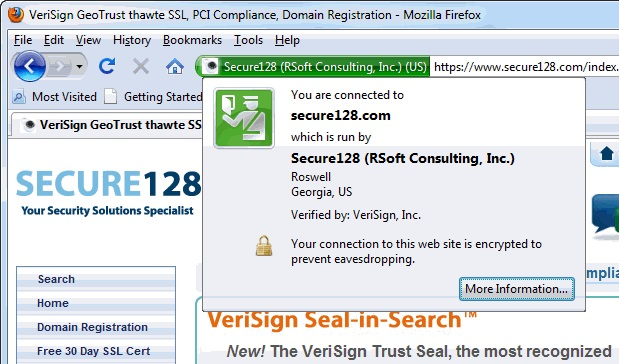
\includegraphics[width=\textwidth, height=0.25\paperheight, keepaspectratio]{../figure/certificate.jpg}
\caption{When you connect to a webpage protected by SSL/TLS, the
Browswer displays information on the certificate's authenticity}
\label{tmplabelfig}
\end{figure}

\begin{figure}
\centering
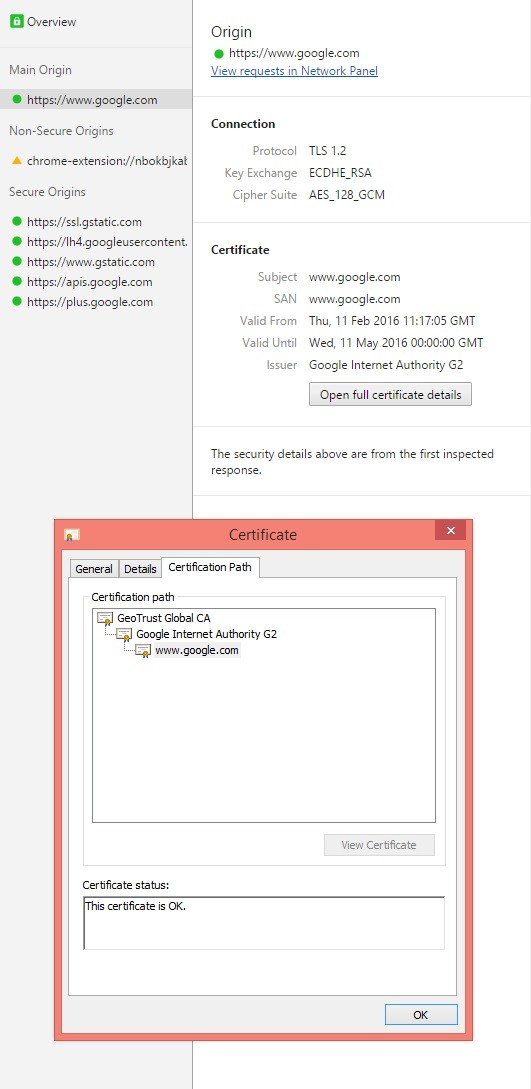
\includegraphics[width=\textwidth, height=0.25\paperheight, keepaspectratio]{../figure/googletls.jpg}
\caption{The cipher and certificate used by '`'Google.com''\,'. Note
that Google has a 2048bit RSA signature key which it then uses to
authenticate an elliptic curve based Diffie-Hellman key exchange
protocol to create session keys for the block cipher AES with 128 bit
key in Galois Counter Mode.}
\label{tmplabelfig}
\end{figure}

\begin{figure}
\centering
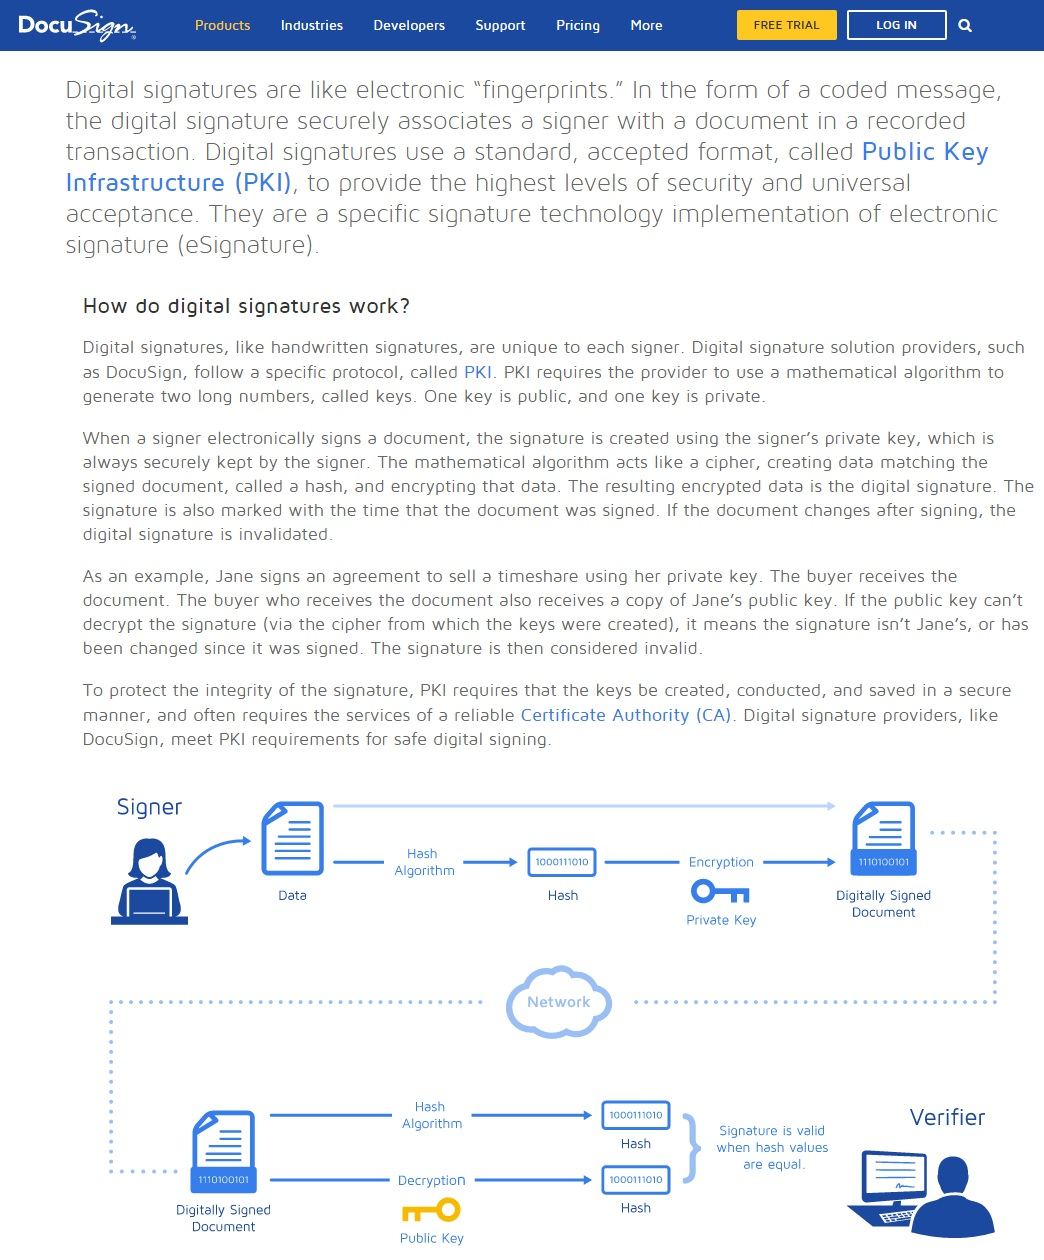
\includegraphics[width=\textwidth, height=0.25\paperheight, keepaspectratio]{../figure/docusign.jpg}
\caption{Digital signatures and other forms of electronic signatures are
legally binding in many jurisdictions. This is some material from the
website of the electronic signing company DocuSign.}
\label{tmplabelfig}
\end{figure}

\begin{quote}
\textbf{Example:} Here is the list of certificate authorities that were
trusted by default (as of spring 2016) by Mozilla products: Actalis,
Amazon, AS Sertifitseerimiskeskuse (SK), Atos, Autoridad de
Certificacion Firmaprofesional, Buypass, CA Disig a.s., Camerfirma,
Certicámara S.A., Certigna, Certinomis, certSIGN, China Financial
Certification Authority (CFCA), China Internet Network Information
Center (CNNIC), Chunghwa Telecom Corporation, Comodo, ComSign, Consorci
Administració Oberta de Catalunya (Consorci AOC, CATCert), Cybertrust
Japan / JCSI, D-TRUST, Deutscher Sparkassen Verlag GmbH (S-TRUST,
DSV-Gruppe), DigiCert, DocuSign (OpenTrust/Keynectis), e-tugra, EDICOM,
Entrust, GlobalSign, GoDaddy, Government of France (ANSSI, DCSSI),
Government of Hong Kong (SAR), Hongkong Post, Certizen, Government of
Japan, Ministry of Internal Affairs and Communications, Government of
Spain, Autoritat de Certificació de la Comunitat Valenciana (ACCV),
Government of Taiwan, Government Root Certification Authority (GRCA),
Government of The Netherlands, PKIoverheid, Government of Turkey, Kamu
Sertifikasyon Merkezi (Kamu SM), HARICA, IdenTrust, Izenpe S.A.,
Microsec e-Szignó CA, NetLock Ltd., PROCERT, QuoVadis, RSA the Security
Division of EMC, SECOM Trust Systems Co.~Ltd., Start Commercial
(StartCom) Ltd., Swisscom (Switzerland) Ltd, SwissSign AG, Symantec /
GeoTrust, Symantec / Thawte, Symantec / VeriSign, T-Systems
International GmbH (Deutsche Telekom), Taiwan-CA Inc.~(TWCA),
TeliaSonera, Trend Micro, Trustis, Trustwave, TurkTrust, Unizeto Certum,
Visa, Web.com, Wells Fargo Bank N.A., WISeKey, WoSign CA Limited
\end{quote}

\section{Appendix: An alternative proof of the density of
primes}\label{10-Appendix-An-alternativ}

I record here an alternative way to show that the fraction of primes in
\([2^n]\) is \(\Omega(1/n)\).\footnote{It might be that the two ways are
  more or less the same, as if we open up the polynomial \((1-x)^kx^k\)
  we get the binomial coefficients.}

\hypertarget{densityprimesaltlem}{}
\begin{lemma} \label[lemma]{densityprimesaltlem}

The probability that a random \(n\) bit number is prime is at least
\(\Omega(1/n)\).

\end{lemma}

\begin{proof} \label[proof]{10-Let-Nn-We-need-to-show}

Let \(N=2^n\). We need to show that the number of primes between \(1\)
and \(N\) is at least \(\Omega(N/\log N)\). Consider the number
\(\binom{2N}{N}=\tfrac{2N!}{N!N!}\). By Stirling's formula we know that
\(\log \binom{2N}{N} = (1 - o(1))2N\) and in particular
\(N \leq \log\binom{2N}{N} \leq 2N\). Also, by the formula using
factorials, all the prime factors of \(\binom{2N}{N}\) are between \(0\)
and \(2N\), and each factor \(P\) cannot appear more than
\(k=\floor{\tfrac{\log 2N}{\log P}}\) times. Indeed, for every \(N\),
the number of times \(P\) appears in the factorization of \(N!\) is
\(\sum_i \floor{\tfrac{N}{P^i}}\), since we get \(\floor{\tfrac{N}{P}}\)
times a factor \(P\) in the factorizations of \(\{1,\ldots,N\}\),
\(\floor{\tfrac{N}{P^2}}\) times a factor of the form \(P^2\), etc.
Thus, the number of times \(P\) appears in the factorization of
\(\binom{2N}{N}=\tfrac{(2N)!}{N!N!}\) is equal to
\(\sum_i \floor{\tfrac{2N}{P^i}}-2\floor{\tfrac{N}{P^i}}\): a sum of at
most \(k\) elements (since \(P^{k+1}>2N\)) each of which is either \(0\)
or \(1\).

Thus,
\(\binom{2N}{N} \leq \prod_{\substack{1 \leq P \leq 2N \\ P \text{ prime }}} P^{\floor{\tfrac{\log 2N}{\log P}}}\).
Taking logs we get that
\begin{equation*}
N \leq \log \binom{2N}{N}
\end{equation*}

\begin{equation*}
\leq \sum_{P \text{ prime} \in [2n]} \floor{\tfrac{\log 2N}{\log P}}\log P
\end{equation*}

\begin{equation*}
\leq \sum_{P \text{ prime} \in [2n]} \log 2N
\end{equation*}
establishing that the number of primes in \([1,N]\) is
\(\Omega(\tfrac{N}{\log N})\).

\end{proof}

\section{Additional Group Theory Exercises and
Proofs}\label{10-Additional-Group-Theor}

Below are optional group theory related exercises and proofs meant to
help gain an intuition with group theory. Note that in this class, we
tend only to talk about finite commutative groups \(\mathbb{G}\), but
there are more general groups:

\begin{itemize}
\item
  For example, the integers (i.e.~infinitely many elements) where the
  operation is addition is a commutative group: if \(a,b,c\) are
  integers, then \(a+b = b+a\) (commutativity), \((a+b)+c = a+(b+c)\)
  (associativity), \(a+0 = a\) (so \(0\) is the identity element here;
  we typically think of the identity as \(1\), especially when the group
  operation is multiplication), and \(a+(-a) = 0\) (i.e.~for any
  integer, we are allowed to think of its additive inverse, which is
  also an integer).
\item
  A non-commutative group (or a non-abelian group) is a group such that
  \(\exists a,b \in \mathbb{G}\) but \(a * b \neq b * a\) (where \(*\)
  is the group operation). One example (of an infinite, non-commutative
  group) is the set of \(2 \times 2\) matrices (over the real numbers)
  which are invertible, and the operation is matrix multiplication. The
  identity element is the traditional identity matrix, and each matrix
  has an inverse (and the product of two invertible matrices is still
  invertible), and matrix multiplication satisfies associativity.
  However, matrix multiplication here need not satisfy commutativity.
\end{itemize}

In this class, we restrict ourselves to finite commutative groups to
avoid complications with infinite group orders and annoyances with
non-commutative operations. For the problems below, assume that a
``group'' is really a ``finite commutative group''.

Here are five more important groups used in cryptography other than
\(\mathbb{Z}_{p}\). Recall that groups are given by a set and a binary
operation.

\begin{itemize}
\tightlist
\item
  For some prime \(p\), \(\mathbb{Z}_p^{\*}=\{1,\ldots , p-1\}\), with
  operation multiplication mod \(p\) (Note: the \(^{\*}\) is to
  distinguish this group from \(\mathbb{Z}_p\) with an additive
  operation and from \(\ensuremath{\mathit{GF}}(p)\).)
\item
  The quadratic residues of \(\mathbb{Z}_p^{\*}\):
  \(Q_p=\{a^2:a\in \mathbb{Z}_p^{\*}\}\) with operation multiplication
  mod \(p\)
\item
  \(\mathbb{Z}_n^{\*}\), where \(n=p\cdot q\) (product of two primes)
\item
  The quadratic residues of \(\mathbb{Z}_n^{\*}\)::
  \(Q_n=\{a^2:a\in \mathbb{Z}_n^{*}\}\), where \(n=p\cdot q\)
\item
  Elliptic curve groups
\end{itemize}

For more familiarity with group definitions, you could verify that the
first 4 groups satisfy the group axioms. For cryptography, two
operations need be efficient for elements \(a,b\) in group
\(\mathbb{G}\): * Exponentiation: \(a,b\mapsto a^b\). This is done
efficiently using repeated squaring, i.e.~generate all the squares up to
\(2^k\) and then use the binary representation. * Inverse:
\(a \mapsto a^{-1}\). This is done efficiently in \(\mathbb{Z}_p^{\*}\)
by Fermat's little theorem. \(a^{-1}=a^{p-2}\) mod \(p\).

\subsection{Solved exercises:}\label{10-Solved-exercises}

\hypertarget{grouptheoryex1}{}
\begin{solvedexercise} \label[solvedexercise]{grouptheoryex1}

Is the set \(S = \{1,2,3,4,5,6\}\) a group if the operation is
multiplication mod \(7\)? What if the operation is addition mod \(7\)?

\end{solvedexercise}

\begin{solution} \label[solution]{10-Yes-if-multiplication-}

Yes (if multiplication) and no (if addition). To prove that something is
a group, we run through the definition of a group. This set is finite,
and multiplication (even multiplication mod some number) will satisfy
commutativity and associativity. The identity element is \(1\) because
any number times \(1\), even mod \(7\), is still itself. To find
inverses, we can in this case literally find the inverses.
\(1 * 1 \mod 7 = 1 \mod 7\) (so the inverse of \(1\) is \(1\)).
\(2 * 4 \mod 7 = 8 \mod 7 = 1 \mod 7\) (so the inverse of \(2\) is
\(4\), and from commutativity, the inverse of \(4\) is \(2\)).
\(3 * 5 \mod 7 = 15 \mod 7 = 1 \mod 7\) (so the inverse of \(3\) is
\(5\), and the inverse of \(5\) is \(3\)).
\(6 * 6 \mod 7 = 36 \mod 7 = 1 \mod 7\) (so \(6\) is its own inverse;
notice that an element can be its own inverse, even if it is not the
identity \(1\)). The set \(S\) is not a group if the operation is
addition for many reasons: one way to see this
\(1+6 \mod 7 = 0 \mod 7\), but \(0\) is not an element of \(S\), so this
group is not \emph{closed} under its operation (implicit in the
definition of a group is the idea that a group's operation must send two
group elements to another element \emph{within the same set of group
elements}).

\end{solution}

\hypertarget{grouptheoryex2}{}
\begin{solvedexercise} \label[solvedexercise]{grouptheoryex2}

What are the generators of the group \(\{1,2,3,4,5,6 \}\), where the
operation is multiplication mod \(7\)?

\end{solvedexercise}

\begin{solution} \label[solution]{10--and--Recall-that-a-ge}

\(3\) and \(5\). Recall that a generator of a group is an element \(g\)
such that \(\{g,g^2,g^3,\cdots\}\) is the entire group. We can directly
check the elements here: \(\{1,1^2,1^3,\cdots\} = \{1\}\), so \(1\) is
not a generator. \(2\) is not a generator because
\(2^3 \mod 7 = 8 \mod 7 = 1\), so the set \(\{2,2^2,2^3,2^4,\cdots\}\)
is really the set \(\{2,4,1\}\), which is not the entire group. \(3\)
will be a generator because \(3^2 \mod 7 = 9 \mod 7 = 2 \mod 7\),
\(3^3 \mod 7 = 2*3 \mod 7 = 6 \mod 7\),
\(3^3 \mod 7 = 18 \mod 7 = 4 \mod 7\), \(3^4 = 12 \mod 7 = 5\),
\(3^5 \mod 7 = 15 \mod 7 = 1\), so
\(\{3,3^2,3^3,3^4,3^5,3^6,3^7 \} = \{3,2,6,4,5,1\}\), which are all of
the elements. \(4\) is not a generator because
\(4^3 \mod 7 = 64 \mod 7 = 1 \mod 7\), so just like \(2\), we won't get
every element. \(5\) is a generator because
\(5^2 \mod 6 = 4, 5^3 \mod 7 = 20 \mod 7 = 6, 5^4 \mod 7 = 30 \mod 7 = 2, 5^5 \mod 7 = 10 \mod 7 = 3, 5^6 \mod 7 = 15 \mod 7 = 1\),
so just like \(3\), \(5\) is a generator. \(6\) is not a generator
because \(6^2 \mod 7= 1 \mod 7\), so just like \(2\), the set
\(\{6,6^2,6^3,\cdots\}\) cannot contain all elements (it will just have
\(1\) and \(6\)).

\end{solution}

\hypertarget{groupex3}{}
\begin{solvedexercise} \label[solvedexercise]{groupex3}

What is the order of every element in the group \(\{1,2,3,4,5,6 \}\),
where the operation is multiplication mod \(7\)?

\end{solvedexercise}

\begin{solution} \label[solution]{10-The-orders-of--are----}

The orders (of \(1,2,3,4,5,6\)) are \(1,3, 6, 3, 6, 2\), respectively.
This can be seen from the work of the previous problem, where we test
out powers of elements. Notice that all of these orders divide the
number of elements in our group. This is not a coincidence, and it is an
example of Lagrange's Theorem, which states that the size of every
subgroup of a group will divide the order of a group. Recall that a
subgroup is simply a subset of the group which is a group in its own
right and is closed under the operation of the group.

\end{solution}

\hypertarget{groupex4}{}
\begin{solvedexercise} \label[solvedexercise]{groupex4}

Suppose we have some (finite, commutative) group \(\mathbb{G}\). Prove
that the inverse of any element is unique (i.e.~prove that if
\(a \in \mathbb{G}\), then if \(b,c \in \mathbb{G}\) such that
\(ab = 1\) and \(ac = 1\), then \(b=c\)).

\end{solvedexercise}

\begin{solution} \label[solution]{10-Suppose-that-a-in-math}

Suppose that \(a \in \mathbb{G}\) and that \(b,c \in \mathbb{G}\) such
that \(ab = 1\) and \(ac = 1\). Then we know that \(ab = ac\), and then
we can apply \(a^{-1}\) to both sides (we are guaranteed that \(a\) has
SOME inverse \(a^{-1}\) in the group), and so we have
\(a^{-1}ab = a^{-1}ac\), but we know that \(a^{-1}a = 1\) (and we can
use associativity of a group), so \((1)b = (1)c\) so \(b = c\). QED.

\end{solution}

\hypertarget{groupex5}{}
\begin{solvedexercise} \label[solvedexercise]{groupex5}

Suppose we have some (finite, commutative) group \(\mathbb{G}\). Prove
that the identity element is unique (i.e.~if \(ca = c\) for all
\(c \in \mathbb{G}\) and if \(cb = c\) for all \(c \in \mathbb{G}\),
then \(a=b\)).

\end{solvedexercise}

\begin{solution} \label[solution]{10-Suppose-that-ca--c-for}

Suppose that \(ca = c\) for all \(c \in \mathbb{G}\) and that \(cb = c\)
for all \(c \in \mathbb{G}\). Then we can say that \(ca =c = cb\) (for
any \(c\), but we can choose some \(c\) in particular, we could have
picked \(c=1\)). And then \(c\) has some inverse element \(c^{-1}\) in
the group, so \(c^{-1}ca = c^{-1}cb\), but \(c^{-1}c = 1\), so \(a = b\)
as desired. QED

\end{solution}

The next few problems are related to quadratic residues, but these
problems are a bit more general (in particular, we are considering some
group, and a subgroup which are all of the elements of the first group
which are squares)

\hypertarget{quadresidueex1}{}
\begin{solvedexercise} \label[solvedexercise]{quadresidueex1}

Suppose that \(\mathbb{G}\) is some (finite, commutative) group, and
\(\mathbb{H}\) is the set defined by
\(\mathbb{H} := \{ h \in \mathbb{G}: \exists g \in G, g^2 = h\}\).
Verify that \(\mathbb{H}\) is a subgroup of \(\mathbb{G}\).

\end{solvedexercise}

\begin{solution} \label[solution]{10-To-be-a-subgroup-we-ne}

To be a subgroup, we need to make sure that \(\mathbb{H}\) is a group in
its own right (in particular, that it contains the identity, that it
contains inverses, and that it is closed under multiplication;
associativity and commutativity follow because we are within a larger
set \(\mathbb{G}\) which satisfies associativity and commutativity).
\emph{Identity} Well, \(1^2 = 1\), so \(1 \in \mathbb{H}\), so
\(\mathbb{H}\) has the identity element. \emph{Inverses} If
\(h \in \mathbb{H}\), then \(g^2 = h\) for some \(g \in \mathbb{G}\),
but \(g\) has an inverse in \(\mathbb{G}\), and we can look at
\(g^2(g^{-1})^2 = (gg^{-1})^2 = 1^2 = 1\) (where I used commutativity
and associativity, as well as the definition of the inverse). It is
clear that \((g^{-1})^2 \in \mathbb{H}\) because there exists an element
in \(\mathbb{G}\) (specifically, \(g^{-1}\)) whose square is
\((g^{-1})^2\). Therefore \(h\) has an inverse in \(\mathbb{H}\), where
if \(h=g^2\), then \(h^{-1} = (g^{-1})^2\). \emph{Closure under
operation} If \(h_1,h_2 \in \mathbb{H}\), then there exist
\(g_1,g_2 \in \mathbb{G}\) where \(h_1 = (g_1)^2, h_2 = (g_2)^2\). So
\(h_1h_2 = (g_1)^2(g_2)^2 = (g_1g_2)^2\), so \(h_1h_2 \in \mathbb{H}\).
Therefore, \(\mathbb{H}\) is a subgroup of \(\mathbb{G}\).

\end{solution}

\hypertarget{quadresidueex2}{}
\begin{solvedexercise} \label[solvedexercise]{quadresidueex2}

Assume that \(|\mathbb{G}|\) is an even number and is known, and that
\(g^{|\mathbb{G}|}=1\) for any \(g \in \mathbb{G}\). Also assume that
\(\mathbb{G}\) is a cyclic group, i.e.~there is some
\(g \in \mathbb{G}\) such that any element \(f \in \mathbb{G}\) can be
written as \(f^k\) for some integer \(k\). Also assume that
exponentiation is efficient in this context (i.e.~we can compute \(g^r\)
for any \(0 \leq r \leq |\mathbb{G}|\) in an efficient time for any
\(g \in \mathbb{G}\)).

Under the assumptions stated above, prove that there is an efficient way
to check if some element of \(\mathbb{G}\) is also an element of
\(\mathbb{H}\), where \(\mathbb{H}\) is still the subgroup of squares of
elements of \(\mathbb{G}\) (note: running through all possible elements
of \(\mathbb{G}\) may not be efficient, so this cannot be your
strategy).

\end{solvedexercise}

\begin{solution} \label[solution]{10-Suppose-that-we-receiv}

Suppose that we receive some element \(g \in \mathbb{G}\). We want to
know if there exists some \(g' \in \mathbb{G}\) such that \(g = (g')^2\)
(this is equivalent to \(g\) being in \(\mathbb{H}\)). To do so, compute
\(g^{|\mathbb{G}|/2}\). I claim that \(g^{|\mathbb{G}|/2}=1\) if and
only if \(g \in \mathbb{H}\).

(Proving the if): If \(g \in \mathbb{H}\), then \(g=(g')^2\) for some
\(g' \in \mathbb{G}\). We then have that
\(g^{|\mathbb{G}|/2} = ((g')^2)^{|\mathbb{G}|/2} = (g')^{|\mathbb{G}|}\).
But from our assumption, an element raised to the order of the group is
\(1\), so \((g')^{|\mathbb{G}|} = 1\), so \(g^{|\mathbb{G}|/2} = 1\). As
a result, if \(g \in \mathbb{H}\), then \(g^{|\mathbb{G}|/2} = 1\).

(Proving the only if): Now suppose that \(g^{|\mathbb{G}|/2} = 1\). At
this point, we use the fact that \(\mathbb{G}\) is cyclic, so let
\(f \in \mathbb{G}\) be the generator of \(\mathbb{G}\). We know that
\(g\) is some power of \(f\), and this power is either even or odd. If
the power is even, we are done. If the power is odd, then
\(g = f^{2k+1}\) for some natural number \(k\). And then we see
\(g^{|\mathbb{G}|/2} = (f^{2k+1})^{|\mathbb{G}|/2} = f^{|\mathbb{G}| + |\mathbb{G}|/2} = f^{|\mathbb{G}|}f^{|\mathbb{G}|/2}\).
We can use the assumption that any element raised to its group's order
is \(1\), so
\(1 = g^{|\mathbb{G}|/2} = f^{|\mathbb{G}|}f^{|\mathbb{G}|/2} = f^{|\mathbb{G}|/2}\).
This tells us that the order of \(f\) is at most \(|\mathbb{G}|/2\), but
this is a contradiction because \(f\) is a generator of \(\mathbb{G}\),
so its order cannot be less than \(|\mathbb{G}|\) (if it were, then
looking at \(\{f,f^2,f^3,\cdots\}\), we would only count at most half of
the elements before cycling back to \(1,f,f^2,\cdots\), so this set
wouldn't contain all of \(\mathbb{G}\)). As a result, we have reached a
contradiction, so \(g^{|\mathbb{G}|/2} = 1\) means that
\(g = f^{2k} = (f^k)^2\), so \(g \in \mathbb{H}\).

We are given that this exponentiation is efficient, so checking
\(g^{|\mathbb{G}|/2} == 1\) is an efficient and correct way to test if
\(g \in \mathbb{H}\). QED.

This proof idea came from
\href{https://crypto.stanford.edu/pbc/notes/numbertheory/qr.html}{here}
as well as from the 2/25/20 lecture at Harvard given by MIT professor
Yael Kalai.

\textbf{Commentary on assumptions and proof}: Proving that
\(g^{|\mathbb{G}|}=1\) is a useful exercise in its own right, but it
overlaps somewhat with our problem sets of 2020, so we will not prove it
here; observe that if \(\mathbb{G}\) is the set of
\(\{1,2,3,\cdots,p-1\}\) for some prime \(p\), then this is a special
case of Fermat's Little Theorem, which states that
\(a^{p-1} \mod p = 1\) for \(a \in \{1,2,3,\cdots,p-1\}\). Also, one can
prove that \(Z_p^{\*}\) (the set of numbers \(0,1,2,\cdots,p-1\), with
operation multiplication mod \(p\)) for \(p\) a prime is cyclic, where
one method can be found
\href{https://crypto.stanford.edu/pbc/notes/numbertheory/gen.html}{here},
where the proof comes down to factorizing certain polynomials and
decomposing numbers in terms of prime powers. We can then see that this
proof above says that there is an efficient way to test whether an
element of \(Z_p^{\*}\) is a square or not.

\end{solution}
